\documentclass[blockchains,review,submit,moreauthors]{Definitions/mdpi}

\usepackage{needspace}
% Use scalable sans-serif fonts for the template's small metadata labels.
\renewcommand{\sfdefault}{lmss}
\usetikzlibrary{arrows.meta,positioning,calc,fit,shapes.geometric}
% Compatibility shim for MiKTeX installations whose LaTeX kernel predates the
% tagging socket used by the current marginnote package. It is inert in the
% submission PDF and is ignored when the current kernel defines the command.
\providecommand\UseTaggingSocket[1]{}
\makeatletter
\@ifundefined{insert@pcolumn}{\let\insert@pcolumn\insert@column}{}
\makeatother
\setlength{\headheight}{20pt}
\newcolumntype{P}[1]{>{\RaggedRight\arraybackslash}p{#1}}
\newcolumntype{Y}{>{\RaggedRight\arraybackslash}X}
\newcommand{\OAL}{\textit{Object--Assurance--Lifecycle} (OAL)}
\newcommand{\CDUTP}{Cross-Domain Unmanned Trust Profile (CDUTP)}

\firstpage{1}
\makeatletter\setcounter{page}{\@firstpage}\makeatother
\pubvolume{1}\issuenum{1}\articlenumber{0}\pubyear{2026}\copyrightyear{2026}
\datereceived{}\daterevised{}\dateaccepted{}\datepublished{}

\Title{Blockchain-Assisted Mission Trust in Air--Surface--Underwater Unmanned Systems: A Cross-Layer Review and Object--Assurance--Lifecycle Framework}
\Author{Anonymous Author(s)}
\AuthorNames{Anonymous Author(s)}
\address{Author affiliations withheld for double-anonymous review}
\corres{Correspondence details withheld for double-anonymous review}

\abstract{Air--surface--underwater missions combine unmanned aerial, surface, and underwater vehicles across heterogeneous links, intermittent connectivity, and administrative domains. A mission decision must combine evidence about physical observations, digital records, shared state, and fitness for use. This narrative review synthesizes literature on cross-domain cooperation, unmanned-system security, trust and reputation, provenance, remote attestation, zero trust, and permissioned blockchains. It proposes the Object--Assurance--Lifecycle (OAL) framework, relating four trust objects (entity, platform/device, link/path, and data product) to four assurance layers (observation validity, commitment and provenance integrity, ledger and governance consistency, and mission-use suitability) across six mission stages. A typed dependency graph and context--temporal--graph reasoning loop separate evidence appraisal from reliance policy and identify where lineage, common causes, and missing evidence affect decisions. A worked example illustrates the resulting acceptance and restriction rules. The synthesis identifies conditional ledger roles in membership, commitments, version coordination, audit, and post-partition reconciliation, with physical validity, endpoint protection, local safety, and governance supported by complementary controls. A claim-specific evidence-maturity profile, research propositions, and a proposed Cross-Domain Unmanned Trust Profile define an evaluation agenda. The framework remains conceptual; comparative performance and integrated mission effectiveness require empirical validation.}
\keyword{mission trust; unmanned systems; UAV--USV--UUV cooperation; blockchain; data provenance; remote attestation; zero trust; maritime autonomy}

\begin{document}

\section{Introduction}

Unmanned maritime operations are becoming systems of systems. A UAV can rapidly survey a wide area and maintain a radio link; a USV can loiter, carry compute and communications equipment, and bridge air and underwater segments; a UUV can collect close-range observations where radio and satellite services do not reach. Cross-domain control studies increasingly coordinate such platforms for search, tracking, formation, navigation, and surveillance missions \citep{hu2024coordinated,wei20233u,wu2020cooperative,ke2022cooperative,liu2023formation,ke2023cross,pang2026cooperative}. The complementary capabilities are operationally attractive, but they also couple domains whose communication physics, failure modes, owners, and security assumptions differ substantially. Broad reviews of UAV networks and applications emphasize mobility, limited energy, intermittent links, and safety constraints \citep{hayat2016survey,shakhatreh2019unmanned,mohsan2023unmanned}; reviews of unmanned marine and underwater vehicles add acoustic delay, difficult localization, harsh deployment conditions, and constrained recovery \citep{bae2023survey,wibisono2023survey,gonzlezgarca2020autonomous}. A mission decision may therefore depend on evidence that has crossed several media, gateways, processing stages, and administrative boundaries.

This creates a \emph{mission-trust gap}. Conventional cybersecurity questions---who authenticated, which packet arrived, whether a file hash matches, or whether replicas agree---remain necessary, yet none alone answers whether a particular data product is suitable for a particular decision at a particular time. A correctly signed sonar report can be physically implausible; a valid observation can be replayed after it becomes stale; a correctly ordered ledger entry can originate from a captured endpoint; and a well-provenanced product can still be unsuitable for a high-consequence task because its uncertainty is too large. Research on UAV and swarm security catalogs spoofing, jamming, routing attacks, capture, malware, data manipulation, and privacy threats \citep{mekdad2023survey,wang2025survey,hadi2023comprehensive,yahuza2021internet}. Underwater-network security reviews describe related attacks under low bandwidth, long propagation delay, and expensive retransmission \citep{jiang2019securing,yang2018challenges,yisa2021security,adam2024state}. These literatures identify important mechanisms, but the unit of analysis is often a platform or network rather than the chain from physical observation to mission use.

Blockchain is frequently proposed as an answer to distributed trust. UAV-oriented reviews report uses in identity, authentication, coordination, access control, data sharing, and audit \citep{hafeez2023blockchain,alladi2020applications,mehta2020blockchain,hawashin2024blockchain,phadke2024unifying}. Representative proposals use ledgers for swarm identity, lightweight authentication, trusted message exchange, and distributed data acquisition \citep{han2022identity,tan2022blockchain,liu2023lightweight,islam2019bus,karmakar2024blockchain}. Maritime reviews similarly associate blockchain with documentation, information sharing, authentication, and inter-organizational coordination \citep{farah2024survey,li2021survey,yang2019maritime}. The attraction is understandable: several organizations can maintain a shared, append-oriented record without granting one participant unilateral control over history. However, the word \emph{trust} becomes ambiguous when replicated-state consistency is allowed to stand for sensor truth, endpoint integrity, privacy, or timeliness. General blockchain security and Internet-of-Things (IoT) surveys repeatedly document scalability, resource, governance, privacy, and interoperability constraints \citep{li2020survey,reyna2018blockchain,uddin2021survey,monrat2019survey}. A useful review must therefore say not only where a ledger helps, but what it does not establish and when it is unnecessary.

Adjacent research offers parts of the answer. Zero trust rejects implicit confidence based only on network location and instead emphasizes explicit, least-privilege, continuously evaluated access \citep{rose2020zero,syed2022zero}. Remote attestation separates the production of device evidence, its appraisal, and the relying party's decision \citep{birkholz2023remote,hardjono2021towards,ott2023universal}. Provenance models describe how entities, activities, and agents are related and can support accountability across transformations \citep{w3c2013provdm,w3c2013provo,hu2020survey,pan2023data}. Trust-management research supplies reputation, probabilistic, subjective-logic, fuzzy, and learning-based methods \citep{ahmed2019trust,aaqib2023iot,junior2021survey,jsang2016subjective,mui2003computational,kamvar2003eigentrust}. Yet these mechanisms are normally discussed in separate architectural vocabularies. A cross-domain mission requires them to be aligned around the objects being judged, the assurance claim being made, and the stage at which evidence is needed.

This review advances one central argument: \emph{mission trust is a chain of non-substitutable assurance claims, and blockchain can strengthen selected transitions in that chain but cannot complete the chain by itself}. To make the argument operational, we propose the authors' \OAL{} framework. It relates four trust objects---entity, platform/device, link/path, and data product---to four assurance layers---observation validity, commitment and provenance integrity, ledger and governance consistency, and mission-use suitability---over six lifecycle stages from admission to recovery. A cross-cutting assurance and governance plane carries identities, attestation results, provenance commitments, trust state, policy and model versions, ledger state, and consortium rules. It is a plane of mechanisms, not a fifth mission object.

The review makes five further contributions. First, it represents dependencies through a typed object graph with relations such as \textit{controls}, \textit{hosts}, \textit{observes}, \textit{transmits}, \textit{transforms}, \textit{endorses}, \textit{records}, and \textit{consumes}. This graph joins evidence propagation to attack propagation. Second, it reframes dynamic trust as a context--temporal--graph (CTG) reasoning loop rather than as a new calibrated algorithm: evidence is appraised, attributed, propagated with uncertainty, converted into a policy action, audited, and fed back. Third, it introduces a unified threat-analysis sentence---attacker, capability, object, propagation path, mission impact, and control---while explicitly separating malice, benign environmental degradation, and insufficient evidence. Fourth, it supplies an evidence-maturity ladder from conceptual argument to sustained deployment. Fifth, it proposes a future \CDUTP{} that maps mission-trust evidence to existing zero-trust, attestation, provenance, communications, and permissioned-ledger specifications. The profile is an author proposal, not a current standard.

The scope is deliberately public and defensive. Civil applications and publicly documented military-support settings are included because coalition ownership, contested communication, and mission criticality sharpen the governance problem. The review does not discuss weapon effects, targeting procedures, or sensitive tactics. It reports no new experiment, dataset, performance result, protocol proof, or calibrated trust score. Its originality lies in conceptual integration, boundary setting, and an evaluation agenda that can be tested by future work.

The remainder of the paper describes the review scope and analytical lens (Section~\ref{sec:scope}), establishes the operational and conceptual foundations, compares fragmented research landscapes, develops OAL and CTG reasoning, examines blockchain patterns and boundaries, organizes evaluation evidence by maturity, and closes with research propositions, limitations, and conclusions.

\section{Review Scope and Analytical Lens}\label{sec:scope}

This narrative review draws on 141 references: 130 scholarly papers and book chapters, one book, and 10 standards, technical reports, or other official technical references. The literature is in English and mainly covers publications from 2016--2026, supplemented by earlier foundational work on reputation, distributed-system limits, provenance, and consensus. The scholarly literature includes original studies, reviews, and papers describing datasets, benchmarks, and simulation platforms.

The references cover six related themes: UAV blockchain and swarm security; maritime and underwater communication and security; heterogeneous UAV--USV--UUV cooperation; IoT trust and reputation; provenance, attestation, and zero trust; and permissioned-ledger architecture and governance. Unmanned-system studies establish the operational constraints of air, surface, and underwater missions. General IoT, cybersecurity, and distributed-systems research provides mechanisms for authentication, evidence appraisal, data sharing, and coordination. Standards and official specifications supply architectural definitions and interoperability requirements, while datasets and simulation platforms provide resources for evaluation.

The analysis compares mechanisms by the object being assessed, the assurance claim they support, and the mission stage at which they operate. These three dimensions form the Object--Assurance--Lifecycle (OAL) framework. Each comparison considers the supporting evidence and the network, resource, threat, and governance assumptions that condition its use. Transfer to a maritime mission depends on whether those assumptions hold in the target environment. For example, a consensus mechanism evaluated on shore servers requires separate assessment under the energy limits and intermittent acoustic connectivity of a UUV. This perspective connects the literature to the dependency analysis, CTG reasoning loop, and evaluation agenda developed in later sections.

Table~\ref{tab:scope} summarizes the review scope. UAVs, USVs, and underwater vehicles form the operational focus, with satellite, shore, cloud, and edge systems providing supporting infrastructure. The lifecycle extends from admission and sensing through mission decisions to audit, revocation, and recovery, encompassing both operational trust and accountability across participating organizations.

\begin{table}[!htbp]
\caption{Review scope and analytical focus.\label{tab:scope}}
\begin{tabularx}{\textwidth}{@{}P{29mm}YY@{}}
\toprule
\textbf{Dimension} & \textbf{Analytical focus} & \textbf{Complementary context}\\
\midrule
Physical domains & UAV, USV, UUV/AUV/ROV; buoys and cross-media gateways & Ground-vehicle analogies and platform structural-certification requirements\\
Infrastructure & Satellite, high-altitude, shore, cloud, edge, and consortium services & Partition-aware operation and explicit infrastructure trust assumptions\\
Mission settings & Observation, inspection, search and rescue, environmental monitoring, logistics, and publicly documented defense-support contexts & Publicly reportable assurance semantics, failure modes, and evaluation methods\\
Trust mechanisms & Identity, authorization, attestation, provenance, dynamic inference, policy, ledger, audit, and governance & Resource requirements, evidence freshness, uncertainty, and conditions for cross-domain use\\
Evidence & Original studies, reviews, a scholarly book, standards, and official technical references & Datasets, benchmarks, simulation platforms, and foundational work from related fields\\
Review output & Conceptual framework, taxonomy, design boundaries, evidence profile, and research propositions & Empirical comparison, formal verification, and deployment certification as evaluation stages\\
\bottomrule
\end{tabularx}
\end{table}

\section{Operational Context and Trust Foundations}

\subsection{A Heterogeneous Mission System of Systems}

The core system contains UAVs, USVs, and UUVs that contribute different sensing, mobility, computation, and communications functions. UAVs offer rapid repositioning, line-of-sight radio relays, and electro-optical sensing, but their payload, endurance, and link stability are constrained. USVs can carry larger energy stores and antennas, remain on station, and bridge acoustic and radio networks. UUVs provide proximity to underwater targets and environments but frequently depend on low-rate acoustic channels, short-range optical links, or delayed surfacing for high-volume transfer. Surveys of UAV-aided maritime communication and 6G maritime connectivity illustrate the relay opportunities \citep{nomikos2023survey,nomikos2024improving}; underwater communication reviews document the trade-offs among acoustic, optical, and other media \citep{ali2020recent,saeed2019underwater,diamant2018low,jahanbakht2021internet}. The resulting system requires a dynamic network model in which topology, latency, bandwidth, clock quality, and reachability can change during a single mission.

Full-text inspection sharpens this point. Civil-UAV communication requirements are explicitly mission-dependent: application classes vary in network role, data volume, range, and quality-of-service needs \citep{hayat2016survey}. Maritime-search evidence characterizes heterogeneous cooperative systems as an early-stage applied field built on increasingly mature UAV, USV, and UUV capabilities \citep{li2023survey}. Mission trust is therefore conditioned on current role and mission phase, with evidence re-evaluated whenever the application domain or consequence changes.

Cross-domain cooperation also changes fault containment. A USV may be the navigation reference, data cache, radio gateway, and permissioned-ledger peer for several UUVs. Compromise or benign failure of that high-betweenness platform therefore affects link evidence, time, provenance continuity, and access to the shared record. Conversely, platform diversity can improve resilience when evidence from independent media and locations can corroborate an event. Cooperation research demonstrates the control and planning value of heterogeneous formations and multi-swarms \citep{stolfi2021uav,xue2021distributed,liu2023formation,ke2023cross}. Mission assurance extends these results by making the trustworthiness of shared observations, commands, and dependencies explicit.

Administrative heterogeneity is equally important. A civil emergency may combine government responders, commercial communications providers, research vehicles, and contracted data services. A coalition mission may include platforms that remain under distinct authorities. Cross-organizational authority therefore combines local authentication with policy equivalence, delegated roles, and accountable governance. The system boundary includes organizations, credentials, data-use restrictions, software and model versions, and the process that admits, suspends, or removes participants. Under these conditions, a shared ledger can provide a consistent audit state whose history is jointly governed by the participating parties.

\begin{figure}[H]
\centering
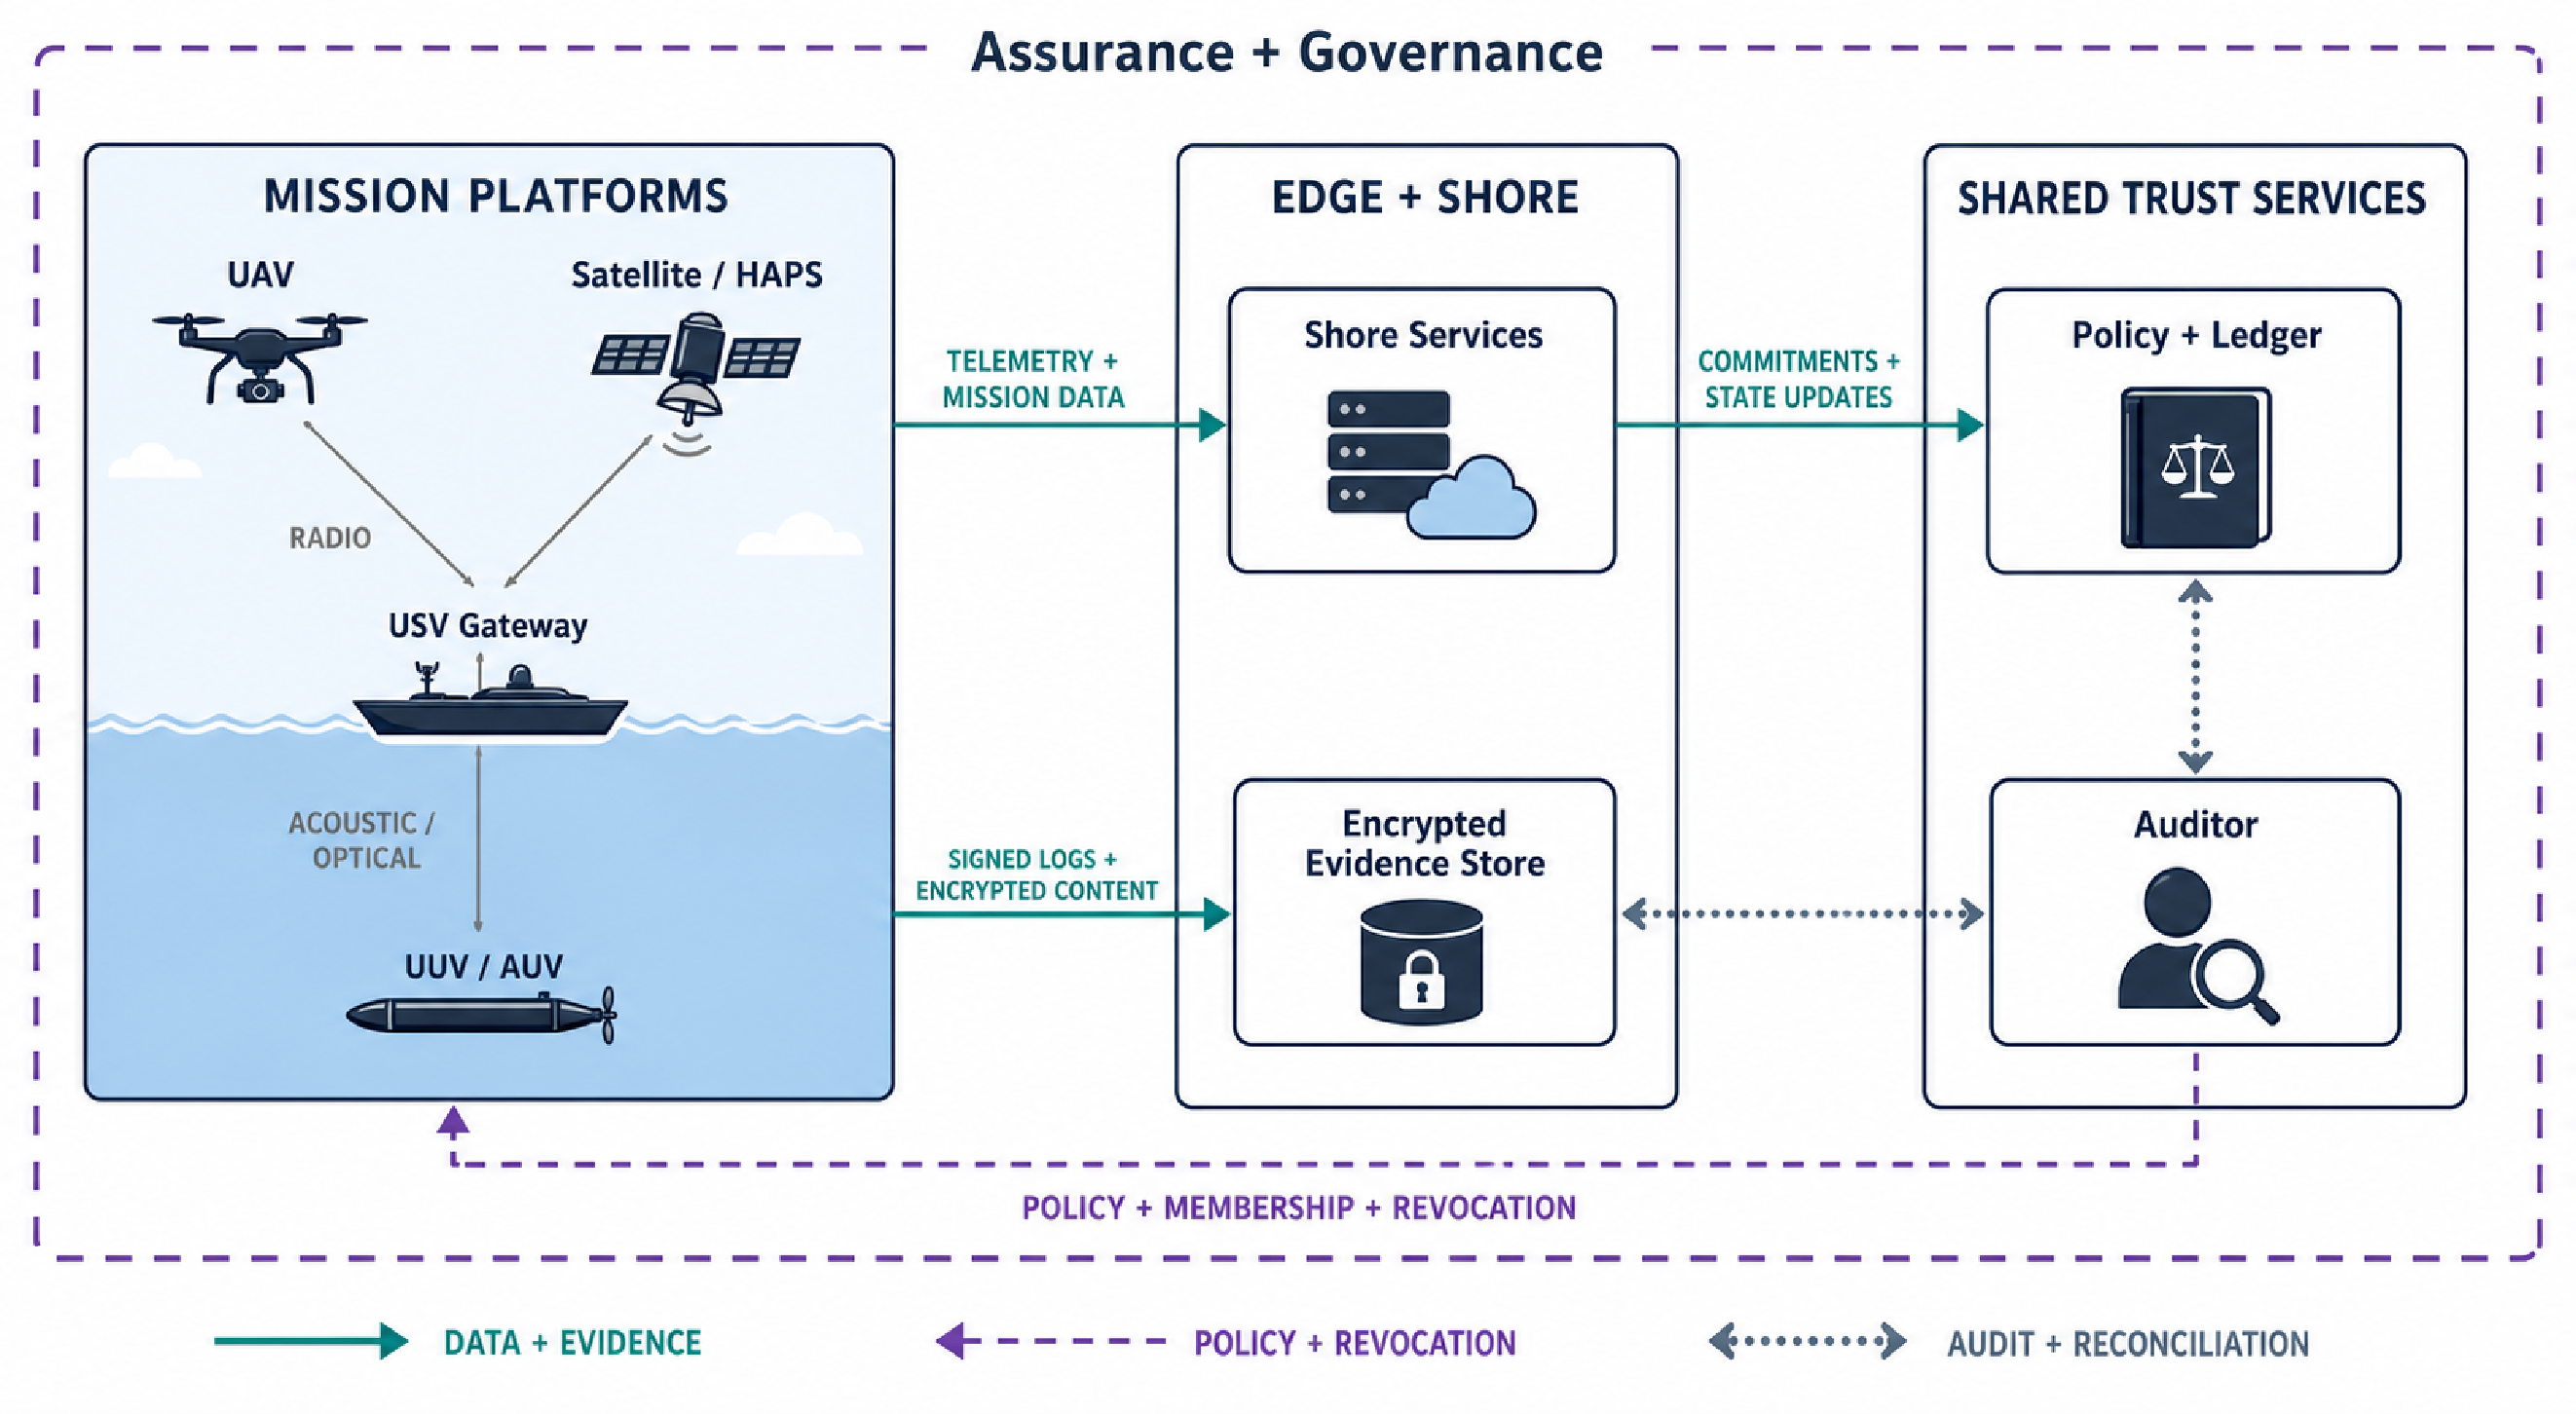
\includegraphics[width=\textwidth]{figures/figure-01-reference-architecture.pdf}
\caption{Author-proposed cross-domain reference architecture. Solid teal arrows show data and evidence moving toward shore and shared services; dashed violet arrows show policy, membership, and revocation returning to mission platforms; dotted slate links show audit and reconciliation. Radio and acoustic/optical media are labeled on neutral topology lines. Constrained platforms retain signed local logs, while capable gateways and shore services forward commitments when connectivity permits. The dashed enclosure identifies the cross-cutting assurance and governance plane.\label{fig:architecture}}
\end{figure}

Figure~\ref{fig:architecture} presents an adaptable logical deployment. Raw imagery, sonar, telemetry, and detailed attestations remain encrypted off chain. A permissioned ledger may retain content identifiers, commitments, coarse-grained state transitions, membership changes, policy and model versions, revocations, and audit decisions. During disconnection, an edge node keeps an append-only signed sequence and later submits a batch commitment. Reconciliation reveals gaps, duplicates, invalid credentials, and conflicting histories; local sensing and control mechanisms retain responsibility for physical interpretation and real-time deadlines.

\subsection{Mission Trust, Trustworthiness, and a Trusted Data Environment}

We define \emph{mission trust} as a context-specific relying decision about whether an object may contribute to a stated mission purpose, given available evidence and the consequences of error. Trust is therefore relational and prospective: a consumer relies on an object for an action. \emph{Trustworthiness} denotes properties that justify such reliance, including identity authenticity, platform integrity, link availability, provenance, freshness, data quality, and accountable governance. Both vary with time and context. The same UAV may be suitable for low-risk environmental imagery while being excluded from time-critical navigation support because its attestation is stale or its location is uncertain.

For an object $o$, time $t$, context $c$, and mission use $m$, a general representation is
\begin{equation}
T_o(t,c,m)=\Pr\!\left(o\text{ satisfies the properties required for }m\mid\mathcal{E}_{1:t},c\right),
\label{eq:trust}
\end{equation}
where $\mathcal{E}_{1:t}$ denotes the direct and indirect evidence currently available. Equation~\eqref{eq:trust} provides a conceptual notation for context-dependent reliance. Implementations may represent the resulting uncertainty through calibrated probabilities, subjective logic, sets, intervals, ordinal states, or decision rules \citep{jsang2016subjective,mui2003computational,kamvar2003eigentrust}. In each representation, uncertainty and evidence lineage remain explicit alongside the trust assessment.

A \emph{trusted data environment} is the socio-technical setting that produces, transports, transforms, shares, and governs evidence and mission data. It includes principals, devices, paths, data products, policies, models, services, and accountability processes. Mission trust is the decision relation exercised within that environment. A tamper-evident catalog strengthens the environment, while mission-use appraisal determines which cataloged item is fit for a particular decision. Zero trust contributes the access-control architecture: NIST's formulation uses policy engines, identity and device evidence, enforcement points, and protected resources \citep{rose2020zero}. Intermittently connected missions add safe degradation and visible evidence staleness to those functions.

\subsection{Four Non-Substitutable Assurance Claims}

The assurance chain in Figure~\ref{fig:assurance-chain} distinguishes four questions. Observation validity asks whether a measurement plausibly represents the physical phenomenon, considering calibration, geometry, environment, sensor health, and corroboration. Commitment and provenance integrity asks who or what produced the item, when and where it was produced, how it was transformed, and whether the recorded bytes and lineage were altered. Ledger and governance consistency asks whether authorized record keepers agree on membership, order, versions, and state transitions under stated fault assumptions. Mission-use suitability asks whether the item is timely, relevant, sufficiently certain, policy-compliant, and proportionate to the consequences of the contemplated action.

\begin{figure}[H]
\centering
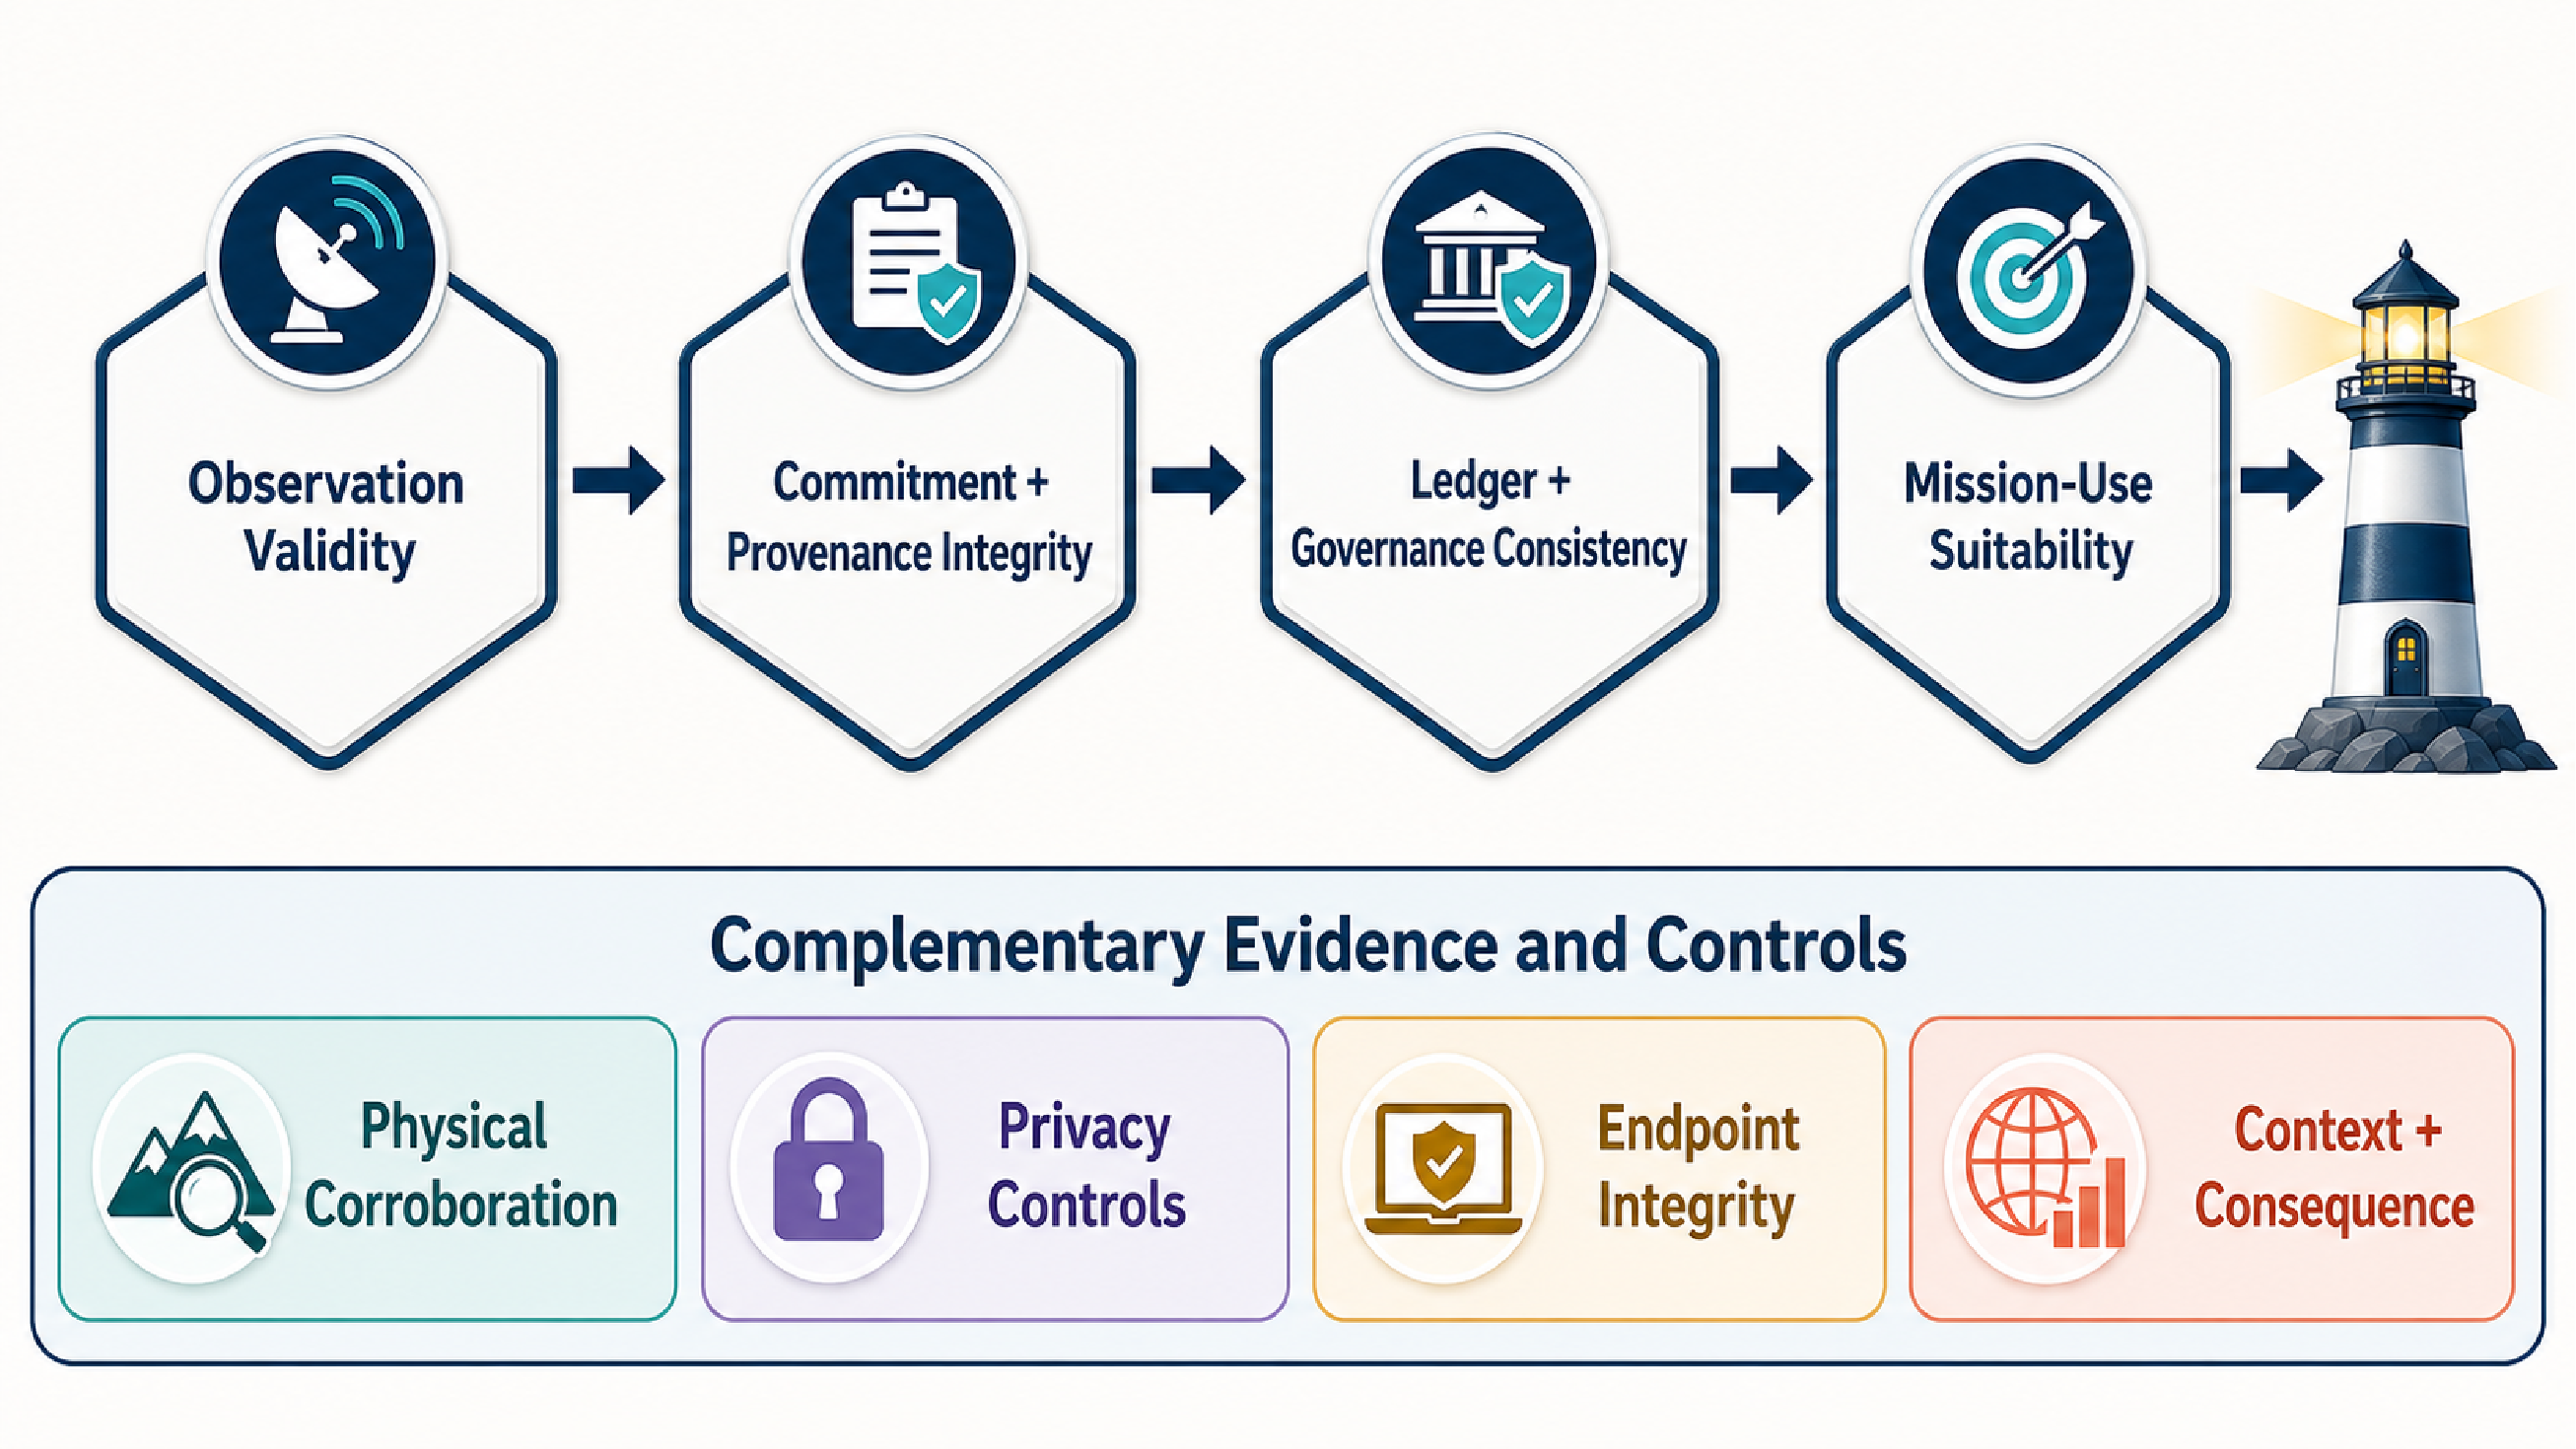
\includegraphics[width=\textwidth]{figures/figure-02-assurance-chain.pdf}
\caption{The authors' four-layer assurance chain. Each layer contributes a distinct claim to the relying decision.\label{fig:assurance-chain}}
\end{figure}

These claims have distinct failure modes. GNSS spoofing can make an otherwise healthy UAV report the wrong location; machine-learning and multi-sensor approaches may detect inconsistency, with validity conditioned on data and context \citep{shafique2021detecting,dang2022deep,semanjski2020use,rado2024recent,varshosaz2019spoofing}. A stolen signing key can produce syntactically valid provenance. A permissioned consensus group can faithfully order false submissions. A delayed but accurate observation can be unfit for collision avoidance. The chain therefore keeps four concepts distinct: signatures and physical truth; hashes and privacy; consensus and endpoint security; and historical reputation and current mission fitness.

Remote attestation and device baselines fit between the first two layers. The RATS architecture distinguishes evidence, appraisal policy, attestation results, and relying parties \citep{birkholz2023remote}; the NIST IoT baseline emphasizes device identification, configuration, data protection, logical access, software update, and cybersecurity-state awareness \citep{fagan2020iot}. These mechanisms justify scoped claims about measured software and device state through roots of trust, reference values, verifier freshness, and explicit measurement coverage. External observation validity is established through complementary physical and sensor evidence. Provenance records derivation: W3C PROV relates entities, activities, and agents, enabling consumers to ask how a product was generated \citep{w3c2013provdm,w3c2013provo}. OAL brings these distinct claims into one mission-oriented vocabulary.

\section{Complementary Research Landscapes}

The relevant literature organizes evidence around different questions: communication performance, cooperative control, adversarial behavior, trust estimation, provenance, and shared-state management. Table~\ref{tab:reviews} maps representative research strands to the mission-assurance questions used in this synthesis. The source-focus column describes the cited literature; the integration column states the authors' proposed cross-domain interpretation. These mappings locate reusable contributions and the assumptions required to combine them. They do not establish a comparative coverage ranking or the absence of a topic from an entire research family.

\begin{table}[!htbp]
\caption{Representative research strands and their role in the OAL synthesis. Integration questions are proposed by the authors; cited sources support the stated research focus.\label{tab:reviews}}
\begin{adjustwidth}{-\extralength}{0cm}
\centering\scriptsize
\begin{tabularx}{\fulllength}{@{}P{32mm}YYP{30mm}@{}}
\toprule
\textbf{Research strand} & \textbf{Source focus} & \textbf{Question for cross-domain integration} & \textbf{Representative sources}\\
\midrule
UAV networks and security & Mission-dependent communication requirements; platform, software, and network threats & Which endpoint and path assumptions accompany an observation or command? & \citep{hayat2016survey,mekdad2023survey,hadi2023comprehensive,wang2025survey}\\
UAV blockchain & Ledger applications, architectures, opportunities, and resource constraints & Which admission, data-sharing, or audit claim requires shared administration? & \citep{hafeez2023blockchain,alladi2020applications,mehta2020blockchain,hawashin2024blockchain}\\
Marine and cross-domain cooperation & Vehicle capabilities, cooperative search, and communication support & How are sensing, planning, and gateway dependencies carried into a relying decision? & \citep{bae2023survey,wibisono2023survey,li2023survey,nomikos2023survey}\\
Underwater communication and security & Channel constraints, reliable collection, threats, and countermeasures & How should delayed or missing evidence affect reliance under both attack and degradation? & \citep{jahanbakht2021internet,jiang2019securing,adam2024state,wei2022reliable}\\
IoT trust and reputation & Evidence aggregation, recommendations, context, and reputation management & What property does an estimate measure, and when does that estimate support mission use? & \citep{ahmed2019trust,aaqib2023iot,junior2021survey,liu2023survey}\\
Provenance, attestation, and zero trust & Data lineage, trust anchors, device appraisal, and resource-access policy & How are origin, measured state, and authorization bound to the same product and decision time? & \citep{syed2022zero,veith2023road,hu2020survey,pan2023data}\\
General IoT blockchain & Integration architectures and computation, storage, communication, and security trade-offs & Which records benefit from replicated governance, and which evidence remains outside the ledger? & \citep{ali2019applications,reyna2018blockchain,uddin2021survey,alladi2019blockchain}\\
\bottomrule
\end{tabularx}
\end{adjustwidth}
\end{table}

\subsection{Cross-Domain Cooperation and Assurance Semantics}

Cooperation studies clarify what platforms can do together. They address formation control, cooperative path planning, and target search across heterogeneous vehicles \citep{wei20233u,wu2020cooperative,ke2022cooperative,xue2021distributed,liu2023formation,pang2026cooperative}. In these control studies, \emph{consensus} denotes convergence or coordination of agent states; replicated-ledger consensus concerns agreement on a shared record state under a specified fault model. The corresponding guarantees apply to different objects and assumptions. OAL proposes to connect a coordination output to security provenance, delegated authority, and cross-organizational audit by treating the output as a data product with traceable inputs, transformation, policy version, and intended mission use.

Maritime search and unmanned-vehicle reviews connect mission capability to sensing, localization, communication, and planning \citep{li2023survey,bae2023survey,gonzlezgarca2020autonomous}. These dependencies motivate claim-specific evidence across platform, path, and data-product states. As illustrative failure cases, a UUV may be healthy while its acoustic path is jammed; a USV gateway may authenticate yet relay a stale model; and UAV imagery may retain authentic pixels while its georegistration is wrong. Each relying decision therefore requires the relevant combination of claims, with the consequences of a failed claim defined for the intended use.

\subsection{From Security Catalogs to Cross-Object Propagation}

UAV, swarm, and underwater-security reviews organize attacks by target and mechanism. Across these domains, reported categories include physical capture, identity and authentication attacks, GNSS spoofing where satellite positioning is used, jamming, denial of service, malicious routing, eavesdropping, malware, false-data injection, and privacy leakage \citep{yahuza2021internet,mekdad2023survey,wang2025survey,jiang2019securing,yang2018challenges}. Hierarchical detection and response provides an example of distributing monitoring and countermeasures in a UAV network \citep{sedjelmaci2018hierarchical}. For OAL, dependency analysis asks how an initial compromise affects subsequent claims. If a captured gateway relays traffic, transforms observations, and holds batch-endorsement keys, a valid ledger commitment may preserve its manipulated output. Effective controls then span the endpoint, transformation, key custody, and ledger interface.

Environmental degradation creates an additional classification problem. Acoustic multipath, Doppler, noise, and changing topology can produce loss, latency, or disagreement; optical links introduce different attenuation and alignment constraints \citep{ali2020recent,saeed2019underwater,jouhari2019underwater,mohsan2022towards}. Such effects can resemble attack. A trust system that equates anomalies with malice may isolate useful nodes during severe conditions, while an adversary may exploit expected environmental variation. A cross-object dependency model should therefore consider both malicious manipulation and benign degradation, including their coexistence, and retain an insufficient-evidence status when the observations cannot distinguish them. Abstention or restricted use can then follow from the uncertainty and mission consequence, without requiring an unsupported diagnosis of malicious intent.

\subsection{Trust Computation with Mission Semantics}

IoT trust and reputation literature provides taxonomies of direct observation, recommendation, context, centralized and distributed management, and attacks on reputation \citep{ahmed2019trust,aaqib2023iot,junior2021survey}; Internet-of-Vehicles work supplies related models under a different mobility and communication setting \citep{hbaieb2022survey}. Underwater studies have explored decision-tree and hidden-Markov approaches \citep{jiang2020dynamic,arifeen2020hidden}, and design guidance recognizes underwater-specific evidence constraints \citep{zhu2024design}. These methods produce classifications or estimates under their model assumptions. Interpreting an output as a calibrated probability of safe mission use requires additional validation. OAL requires each estimate---for example, routing reliability, current software integrity, sensor accuracy, or willingness to cooperate---to name the object, property, context, evidence lineage, uncertainty expression, and permitted use.

Blockchain-based trust-management studies examine shared reputation and tamper-evident updates for IoT and distributed services \citep{liu2023survey,bellini2020blockchain,kumar2022leveraging}, with related designs reviewed in cloud computing \citep{li2021blockchain}. A ledger can make accepted updates auditable under its membership, key-management, and consensus assumptions. It can also preserve misleading recommendations. Collusion, correlated observations, model drift, and incorrect identity binding require evidence appraisal and model validation beyond record integrity. Storage and governance choices therefore follow the definition of the claim and its evidence semantics.

Fog and edge trust approaches place appraisal near constrained devices, while trust-recommendation reviews examine context, recommendation quality, and attack resistance \citep{alkhafajiy2020comitment,mohammadi2019trust}. In a cross-domain mission, a USV edge service may observe several UUVs while remaining their common gateway. Local appraisal can avoid remote communication round trips, but recommendations from that service share dependencies on its platform, clock, path, and administrative owner. Recording those dependencies makes common causes explicit so that aggregation can avoid treating several reports as independent corroboration solely because they concern different vehicles.

\subsection{Provenance, Attestation, and Authorization}

Provenance research provides a vocabulary for origins, transformations, and responsibility \citep{hu2020survey,pan2023data}. W3C PROV represents entities, activities, and agents, with relations for generation, use, derivation, and attribution \citep{w3c2013provdm}. Its terminology needs an explicit mapping: an OAL entity is an acting principal, usually represented as a PROV agent, whereas an OAL data product corresponds to a PROV entity. A provenance description records asserted lineage; reliance on that description additionally requires evidence of trustworthy capture, cryptographic binding, and availability of the referenced records.

Remote attestation addresses a different claim: a verifier appraises evidence about an endpoint, and a relying party uses the resulting assessment. RATS makes the appraisal policy, trust relationships, and freshness conditions explicit \citep{birkholz2023remote}; trust-anchor surveys describe the supporting technologies \citep{veith2023road}. Zero trust supplies principles for resource-specific authentication and authorization using subject, device, and contextual information \citep{rose2020zero,syed2022zero}. OAL connects these mechanisms at decision time: provenance identifies the input and transformation, attestation contributes measured endpoint-state evidence, and authorization identifies permitted reliance. Sensor validity and fitness for a particular physical action still require their own evidence. During disconnection, the integration must specify how long cached assessments and delegated permissions remain usable.

\subsection{Ledger Mechanisms and Physical-Evidence Boundaries}

Blockchain surveys and technical guidance explain architectures, consensus mechanisms, smart contracts, scalability, and security \citep{yaga2018blockchain,wang2019survey,lashkari2021comprehensive,shrimali2022blockchain,hewa2021survey}. IoT integrations confront limited computation, storage, communication, energy, privacy, and interoperability \citep{reyna2018blockchain,dorri2017towards,uddin2021survey}. UAV proposals explore authentication and trusted swarm or network architectures \citep{barka2022towards,jensen2019blockchain,karmakar2024blockchain,zhou2024towards}; maritime transportation proposals address authentication and aggregate signcryption \citep{zhang2022blockchain,yang2022efficient}. These precedents inform choices for membership, key custody, endorsement, validation, and on-chain/off-chain binding. Their relevance to cross-domain missions depends on the tested deployment, connectivity, and threat assumptions; a protocol proposal alone does not demonstrate operational integration across UAVs, USVs, and UUVs.

Cross-sector classifications discuss scalability, integration, and governance problems \citep{casino2019systematic}. Technical guidance also identifies the boundary between recording sensor input and establishing whether it reflects a physical event \citep{yaga2018blockchain}. UAV-specific taxonomies and 6G perspectives motivate evaluating ledger placement against resource, mobility, and network-architecture constraints \citep{kumari2020taxonomy,aggarwal2021blockchain,khan2023swarm}. For the present synthesis, these observations motivate evaluating capable gateways and edge nodes as ledger hosts, together with the new availability and administrative dependencies this placement creates. OAL provides a way to specify the mission-assurance claim that would justify that cost and to compare it with an authenticated non-ledger alternative.

The synthesis opportunity is a common analytical model connecting a physical observation, the responsible principals and devices, the paths and transformations, the shared governance record, and the eventual mission decision. The next section develops that model.

\section{The OAL Framework for Mission Trust}

The \OAL{} framework provides a three-dimensional structure for classification and design. It can be used to locate a published mechanism, specify an assurance requirement, or identify an unprotected transition. The object dimension identifies \emph{what is judged}; the assurance dimension identifies \emph{which claim is sought}; and the lifecycle dimension identifies \emph{when the claim is needed}. These axes are conceptually distinct; evidence and failures across their cells can be dependent. A mechanism may occupy several cells, and some object--claim combinations are inapplicable to a particular mission. The framework organizes an assurance case by locating applicable claims; completeness and effectiveness require evidence about the relevant dependencies and outcomes. Figure~\ref{fig:oal} presents the framework.

\begin{figure}[!htbp]
\centering
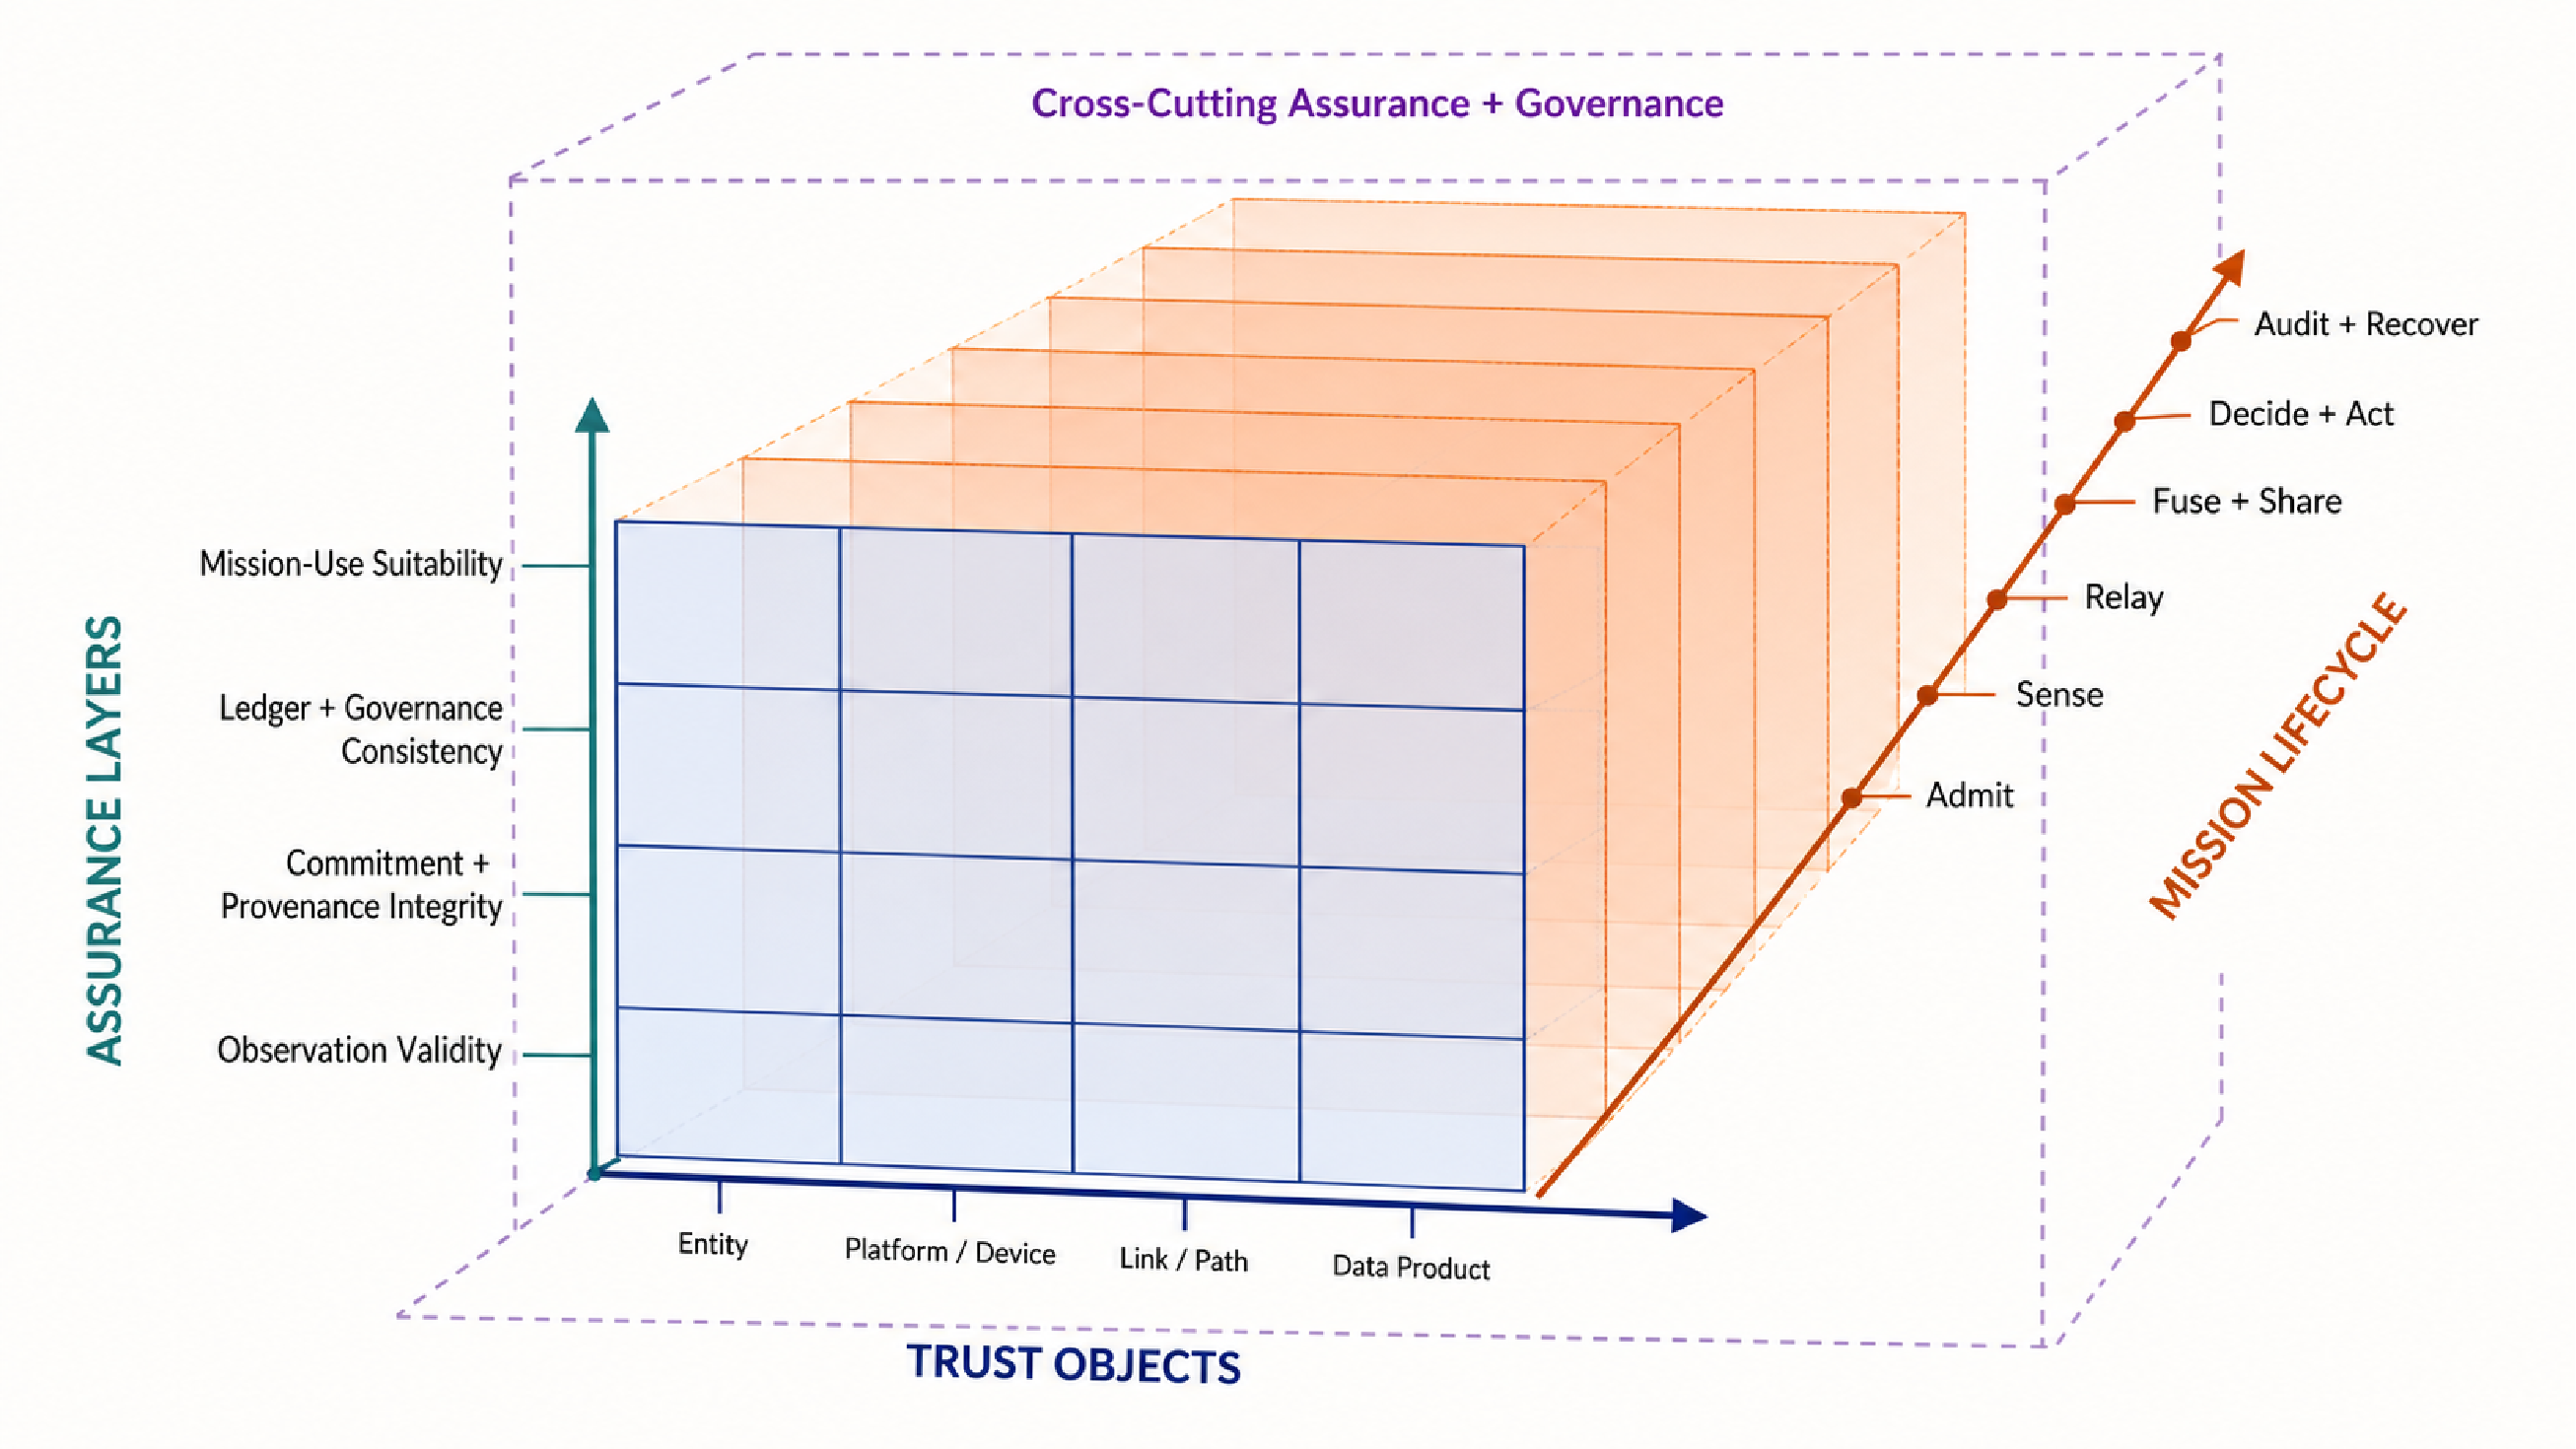
\includegraphics[width=\textwidth]{figures/figure-03-oal-framework.pdf}
\caption{OAL framework for mission trust. Trust objects run along the horizontal front-face axis, assurance layers along the vertical axis, and lifecycle stages along the oblique depth axis. Cells distinguish claims and their timing; the cross-cutting assurance and governance plane supplies shared services and dependencies.\label{fig:oal}}
\end{figure}

\subsection{Dimension I: Four Trust Objects}

An \emph{entity} is a principal capable of holding authority or responsibility: an operator, organization, mission service, software agent, or autonomous decision-making principal. A \emph{platform/device} is an executing physical or virtual endpoint: vehicle, sensor, gateway, compute module, secure element, or hosted execution instance. A stored software image or model artifact is a data product; its deployed state is assessed on the hosting endpoint. This distinction matters because an authorized entity can control a compromised device, while a device with valid attestation can execute a legitimate but unsuitable policy. An autonomous vehicle may occupy both categories under different claims: as a delegated principal for action and as an endpoint whose hardware and software state are measured.

A \emph{link/path} is a time-varying end-to-end route composed of its physical media, intermediate nodes, security associations, and quality state. A data product may traverse a UUV acoustic hop, a USV gateway, a satellite backhaul, and a cloud broker; confidentiality, freshness, availability, and routing integrity depend on this composed path. A \emph{data product} is an identified version of a raw observation, feature set, track, map, fused estimate, model output, command, alert, provenance record, or audit artifact. OAL treats a version as logically immutable: a transformation or correction creates a new identifier. This convention identifies versions; protection against storage alteration requires content verification and retained commitments.

\begin{table}[!htbp]
\caption{Four OAL trust objects, evidence, failure examples, and mission questions.\label{tab:objects}}
\begin{adjustwidth}{-\extralength}{0cm}
\small
\begin{tabularx}{\fulllength}{@{}P{25mm}YYY@{}}
\toprule
\textbf{Object} & \textbf{Representative evidence} & \textbf{Illustrative failure or attack} & \textbf{Mission question}\\
\midrule
Entity & Credential chain, organizational role, delegation, authorization, prior accountable actions & Credential theft, insider misuse, collusion, obsolete authority & Who requests, endorses, or consumes the resource, and under which authority?\\
Platform/device & Secure boot measurement, firmware/software version, sensor self-test, configuration, energy and health state & Capture, malware, unsafe configuration, stale reference value, sensor drift & Which endpoint executes, and is its measured state adequate for this use?\\
Link/path & Authentication state, route, delay, loss, signal indicators, neighbor changes, medium and gateway state & Jamming, wormhole, selective forwarding, eavesdropping, benign fading & Through which changing path did evidence pass, and what security and quality properties held?\\
Data product & Signature, timestamp, location, provenance graph, quality metadata, version, calibration and cross-source residuals & False injection, replay, poisoning, misregistration, unauthorized transformation & Where did this version come from, was it altered, and is it timely and suitable?\\
\bottomrule
\end{tabularx}
\end{adjustwidth}
\end{table}

Policies, models, smart contracts, and ledger state map onto the four operational object categories. They are versioned artifacts hosted on devices or represented as data products, while the principals who authorize them remain entities. This stable object set accommodates new mechanisms, and the assurance plane makes their artifacts first-class subjects of versioning, access control, threat analysis, and audit.

\subsection{Dimension II: Four Assurance Layers}

The first layer, \emph{observation validity}, asks whether evidence about the external world is credible. Relevant controls include calibration records, sensor diagnostics, geometry, physical bounds, environmental models, independent modalities, and temporal continuity. Multi-view and multi-sensor fusion can expose disagreement and express uncertainty \citep{holzinger2022information,liu2022trusted,qian2025review}; it can also amplify correlated error or poisoned inputs. Observation assurance therefore documents independence assumptions and combines physical and domain evidence with cryptographic content commitments.

The second layer, \emph{commitment and provenance integrity}, binds an item to recorded assertions about its producer, time, place, transformation, and version. Digital signatures, authenticated channels, secure timestamps, content identifiers, and W3C PROV relations support this layer \citep{w3c2013provdm,w3c2013provo,hu2020survey,pan2023data,singh2019decision}. A valid signature authenticates a statement under its key assumptions; the accuracy of the stated acquisition time or location requires separate evidence. Provenance covers both raw acquisition and model, human, or automated decisions. Decision provenance connects inputs, policy versions, intermediate transformations, and outputs, making later review possible when those records remain retrievable. Its assurance conditions include key custody, clock assumptions, instrumentation completeness, and trustworthy capture of events.

The third layer, \emph{ledger and governance consistency}, concerns shared state and the rules by which administrative parties maintain it. It covers member admission, endorsement, record ordering, validation, version coordination, revocation, dispute handling, and reconciliation. Hyperledger Fabric illustrates an execute--order--validate architecture with identity-aware channels and endorsement policies \citep{androulaki2018hyperledger,hyperledger2026fabric}; other shared-state services can satisfy the applicable functions. A ledger can establish agreement on validated records under a declared fault model. The legitimacy of governance rules, resolution of organizational disputes, and semantic validity of submissions require additional evidence and procedures. For missions using another shared-state architecture, the corresponding database or audit controls define the applicable assurance claims; ledger-specific claims are marked inapplicable.

The fourth layer, \emph{mission-use suitability}, applies a reliance policy to assurance evidence. Freshness, relevance, uncertainty, risk class, legal and organizational policy, available alternatives, and consequence severity are considered. A consumer may accept a low-resolution image for broad situational awareness but require corroborated, current, and accurately georegistered evidence for autonomous maneuver. An implementation assesses the required properties and separately applies the policy that permits, restricts, or defers an action. Authority to use the product requires the applicable authorization.

\subsection{Dimension III: Six Lifecycle Stages}

The lifecycle dimension prevents security from ending at admission. Table~\ref{tab:lifecycle} shows how objects and assurance questions evolve from credentialing to recovery. Evidence can age, dependencies can change, and an initially valid decision can require reassessment.

\begin{table}[!htbp]
\caption{Mission lifecycle and representative OAL assurance tasks.\label{tab:lifecycle}}
\begin{adjustwidth}{-\extralength}{0cm}
\small
\begin{tabularx}{\fulllength}{@{}P{30mm}YYP{38mm}@{}}
\toprule
\textbf{Stage} & \textbf{Primary questions} & \textbf{Evidence and controls} & \textbf{Ledger-relevant state}\\
\midrule
Admission and authentication & Is the entity authorized, and is the joining endpoint in an acceptable measured state? & Credentials, delegation, attestation, configuration baseline, least privilege & Membership, role, attestation-result commitment, policy version\\
Sensing and collection & Does an observation plausibly reflect its stated time, place, modality, and calibration? & Sensor self-test, secure time/location, quality metadata, corroboration & Acquisition commitment and data identifier\\
Transmission and relay & Which path carried the item, and did quality or security conditions change? & Mutual authentication, route and link telemetry, delay/loss context, custody transfer & Signed relay events or batch roots\\
Processing, fusion, and sharing & Which inputs, code, model, parameters, and policies produced this version? & Provenance graph, reproducible transformation identifier, access and usage control & Version, endorsement, access decision, model/policy commitment\\
Decision and action & Is the product fit for the specific mission consequence now? & Uncertainty, freshness, risk policy, alternatives, human review or fail-safe & Decision rationale commitment and responsible principal\\
Audit, revocation, and recovery & What failed, who was affected, what must be invalidated, and how is operation restored? & Incident evidence, credential and model revocation, rollback, re-attestation, after-action review & Revocation state, dispute outcome, reconciled log, recovery version\\
\bottomrule
\end{tabularx}
\end{adjustwidth}
\end{table}

Lifecycle continuity is especially difficult during partitions. During disconnection from a central policy engine, a UUV needs a local authorization envelope: named resources, permitted actions, risk limit, evidence freshness, expiry, and a context-appropriate fallback. Expiry enforcement requires bounded clock uncertainty and rollback-resistant local state, or a policy that reduces authority when those assumptions fail. Local actions are signed and sequenced; reconnecting nodes later disclose commitments and selected evidence. The design distinguishes \emph{continued operation under delegated authority} from \emph{fresh global authorization}; retained evidence supports later audit, while local enforcement constrains actions during disconnection.

\subsection{The Assurance and Governance Plane}

The cross-cutting plane contains identity and authorization, remote attestation, provenance capture, trust inference, policy/model/contract version management, ledger state, and consortium governance. Each component is itself attackable. Identity authorities can be compromised; reference values can be wrong; provenance instrumentation can omit transformations; a trust model can drift or be poisoned; a smart contract can encode an unsafe rule; validators can collude; and governance can deadlock. The plane must therefore be observed through the same OAL lens. For example, a model is a data product with provenance and validation evidence, a deployed instance is hosted on a device, its approval is an entity action, and its use is constrained by lifecycle stage and mission context.

OAL serves as both a diagnostic and a specification template. A blockchain-throughput study maps to ledger-performance cells and prompts complementary observation, endpoint, and mission-use requirements. A firmware-attestation protocol maps to a device claim at admission and prompts a freshness rule for disconnected decision time. For each applicable cell, a specification records the object/version, required property, evidence source and coverage, validity condition, acceptance rule, responsible party, and response to missing evidence. Reviewing identified high-consequence dependency paths then exposes absent or stale evidence. The resulting assurance case has the scope of its modeled paths; broader coverage requires identification and appraisal of additional dependencies.

\section{Evidence Dependencies, Threat Propagation, and Dynamic Reasoning}

\subsection{A Typed Object-Dependency Graph}

OAL classifies claims; a dependency graph records relations relevant to their appraisal. Let $G_t=(V_t,E_t)$ be a time-indexed directed multigraph whose vertices denote the four object types, with version or state-interval identifiers where applicable. Relations have declared source and target types: an entity \textit{controls} a platform; a platform \textit{hosts} another device or a model artifact; a platform \textit{produces} an observation product; a path \textit{transmits} a product; an entity \textit{endorses} or \textit{consumes} a product; and a ledger-record product \textit{commits to} another product. A derived product \textit{depends on} input products through an identified transformation. Each transformation identifier links all inputs, outputs, the executing platform, responsible entity, code/model version, and event-time interval. A W3C PROV serialization can represent that transformation as an activity node \citep{w3c2013provdm}; activities describe relations among the four OAL object types. An OAL entity corresponds to a responsible principal, usually a PROV agent, while a data product corresponds to a PROV entity. Time and version qualifiers are essential. A decision based on model version 4.2 before a rollback requires that version and activity interval to qualify the relation ``UAV-7 hosts model M.''

\begin{figure}[!htbp]
\centering
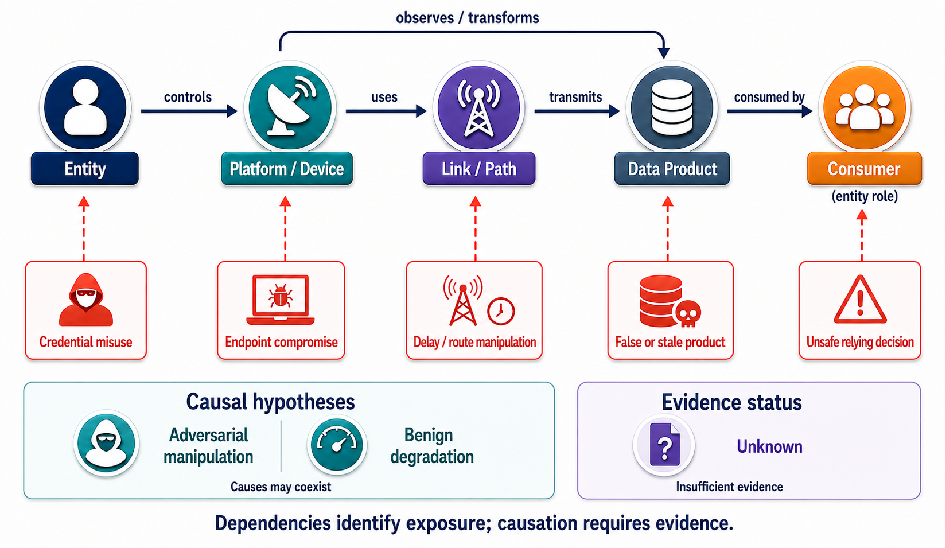
\includegraphics[width=\textwidth]{figures/figure-04-dependency-threat.pdf}
\caption{Simplified object dependencies and illustrative exposures. Solid arrows name operational relations; red dashed arrows associate an exposure with its object. The lower panels distinguish causal hypotheses from the epistemic status of the evidence. Causal propagation claims require explicit causal evidence and inference rules.\label{fig:dependency}}
\end{figure}

The graph supports evidence tracing and exposure analysis. A fresh attestation can support a scoped claim about measured platform state; verified provenance supports recorded derivation; corroborating observations support physical plausibility under their dependence assumptions. Each inference requires an explicit rule connecting evidence to a property. Hosting and transmission relations identify operational dependencies; inference about a property or causal effect requires a specified model. Compromised credentials may permit device access; a compromised device may alter observations; a manipulated path may delay delivery or substitute content if authentication fails; and a consumer may then act on the result. Figure~\ref{fig:dependency} depicts this conditional chain. Traversal follows declared relation semantics to identify claims for reassessment; score updates depend on the specified inference model. If a causal or probabilistic model is used, its conditional structure, common causes, and parameters must be specified separately. Versioning and event ordering expose feedback cycles so that update rules can preserve the identity and dependence of recirculated evidence.

\subsection{A Unified Threat-Analysis Sentence}

Every scenario should be expressible as: \emph{an attacker with capability $C$ acts on object $O$, propagates through relations $P$, creates mission impact $I$, and is constrained or detected by controls $K$ under assumptions $A$}. This grammar connects threat catalogs to assurance cases and exposes missing controls. Table~\ref{tab:threats} applies the grammar to common public scenarios at a capability level suitable for reproducible defensive analysis.

\begin{table}[!htbp]
\caption{Object-centered threat, degradation, and evidence-absence analysis.\label{tab:threats}}
\begin{adjustwidth}{-\extralength}{0cm}
\scriptsize
\begin{tabularx}{\fulllength}{@{}P{24mm}P{29mm}P{34mm}YY@{}}
\toprule
\textbf{Class and initial object} & \textbf{Capability or condition} & \textbf{Propagation path} & \textbf{Mission impact} & \textbf{Controls and residual uncertainty}\\
\midrule
Malicious/entity & Stolen or misused credential & controls device $\rightarrow$ endorses product $\rightarrow$ record accepted & Unauthorized tasking or false accountability & Short-lived delegation, multi-party approval, behavioral evidence, rapid revocation; valid credentials can still mask insider intent\\
Malicious/device & Capture, malware, or model replacement & hosts sensor/model $\rightarrow$ observes/transforms data & Consistent but false products across many consumers & Attestation, key protection, diversity, provenance, quarantine; measured components may omit sensors or runtime behavior\\
Malicious/link & Jamming, wormhole, selective forwarding, replay & transmits/custodies data $\rightarrow$ delays or substitutes version & Loss of availability, stale situational picture, biased fusion & Link context, authenticated sequence, path diversity, freshness policy; attribution remains uncertain\\
Malicious/data & False-data injection, poisoning, semantic manipulation & transformed / endorsed / recorded product $\rightarrow$ consumed decision & Incorrect classification, route, or resource allocation & Physical plausibility, independent modality, robust fusion, lineage; independence assumptions can fail\\
Benign environment & Fading, multipath, weather, occlusion, low energy & environmental conditions degrade link or observation evidence & Delay, disagreement, reduced coverage & Environment-aware baselines, graceful degradation, explicit ``benign-degraded'' hypothesis; models may be incomplete\\
Evidence absence & Disconnection, failed verifier, missing lineage, stale clock & prevents appraisal across several relations & Unsafe overconfidence or unnecessary isolation & Unknown state, bounded authority, conservative policy, later reconciliation; compromise attribution requires additional evidence\\
\bottomrule
\end{tabularx}
\end{adjustwidth}
\end{table}

Three labels organize the interpretation of an anomaly. \emph{Malicious} denotes evidence supporting intentional or adversarial manipulation; \emph{benign-degraded} denotes a supported environmental or operational explanation; and \emph{unknown} denotes insufficient evidence to resolve the explanation. Unknown describes the evidence status of an assessment. Operational states additionally include nominal operation and recovery, and malicious action can coincide with environmental degradation. For example, packet loss may justify restricting reliance on a path, while attribution of attacker intent requires separate support. Recovery tracks review of cached data, keys, neighbors, and prior decisions after software is re-attested. Policies map the assessed properties, uncertainty, and recovery status to bounded actions---continue, reduce privilege, request corroboration, isolate, return, or escalate to a human.

\subsection{The CTG Reasoning Loop}

CTG-Trust is the context--temporal--graph workflow developed in this synthesis and shown in Figure~\ref{fig:ctg}. The workflow specifies inputs and decision records for implementations with selected and validated inference and policy mechanisms. First, evidence events are captured with source, subject, event and receipt times, clock uncertainty, context, value, and lineage. Second, evidence reliability and dependencies are appraised: a device self-report and an external verifier carry different evidential relationships. Third, a selected method assesses a named object property. Fourth, graph traversal identifies downstream claims requiring reassessment and shared causes beyond the local assessment. Fifth, the assessment is revised as needed and its uncertainty made explicit. Sixth, a mission policy chooses an action. Seventh, the decision, relevant versions, and evidence commitment are recorded for review. Eighth, independently appraised outcomes and later verification update the evidence base, with ground-truth labels established independently of the workflow's decisions.

\begin{figure}[!htbp]
\centering
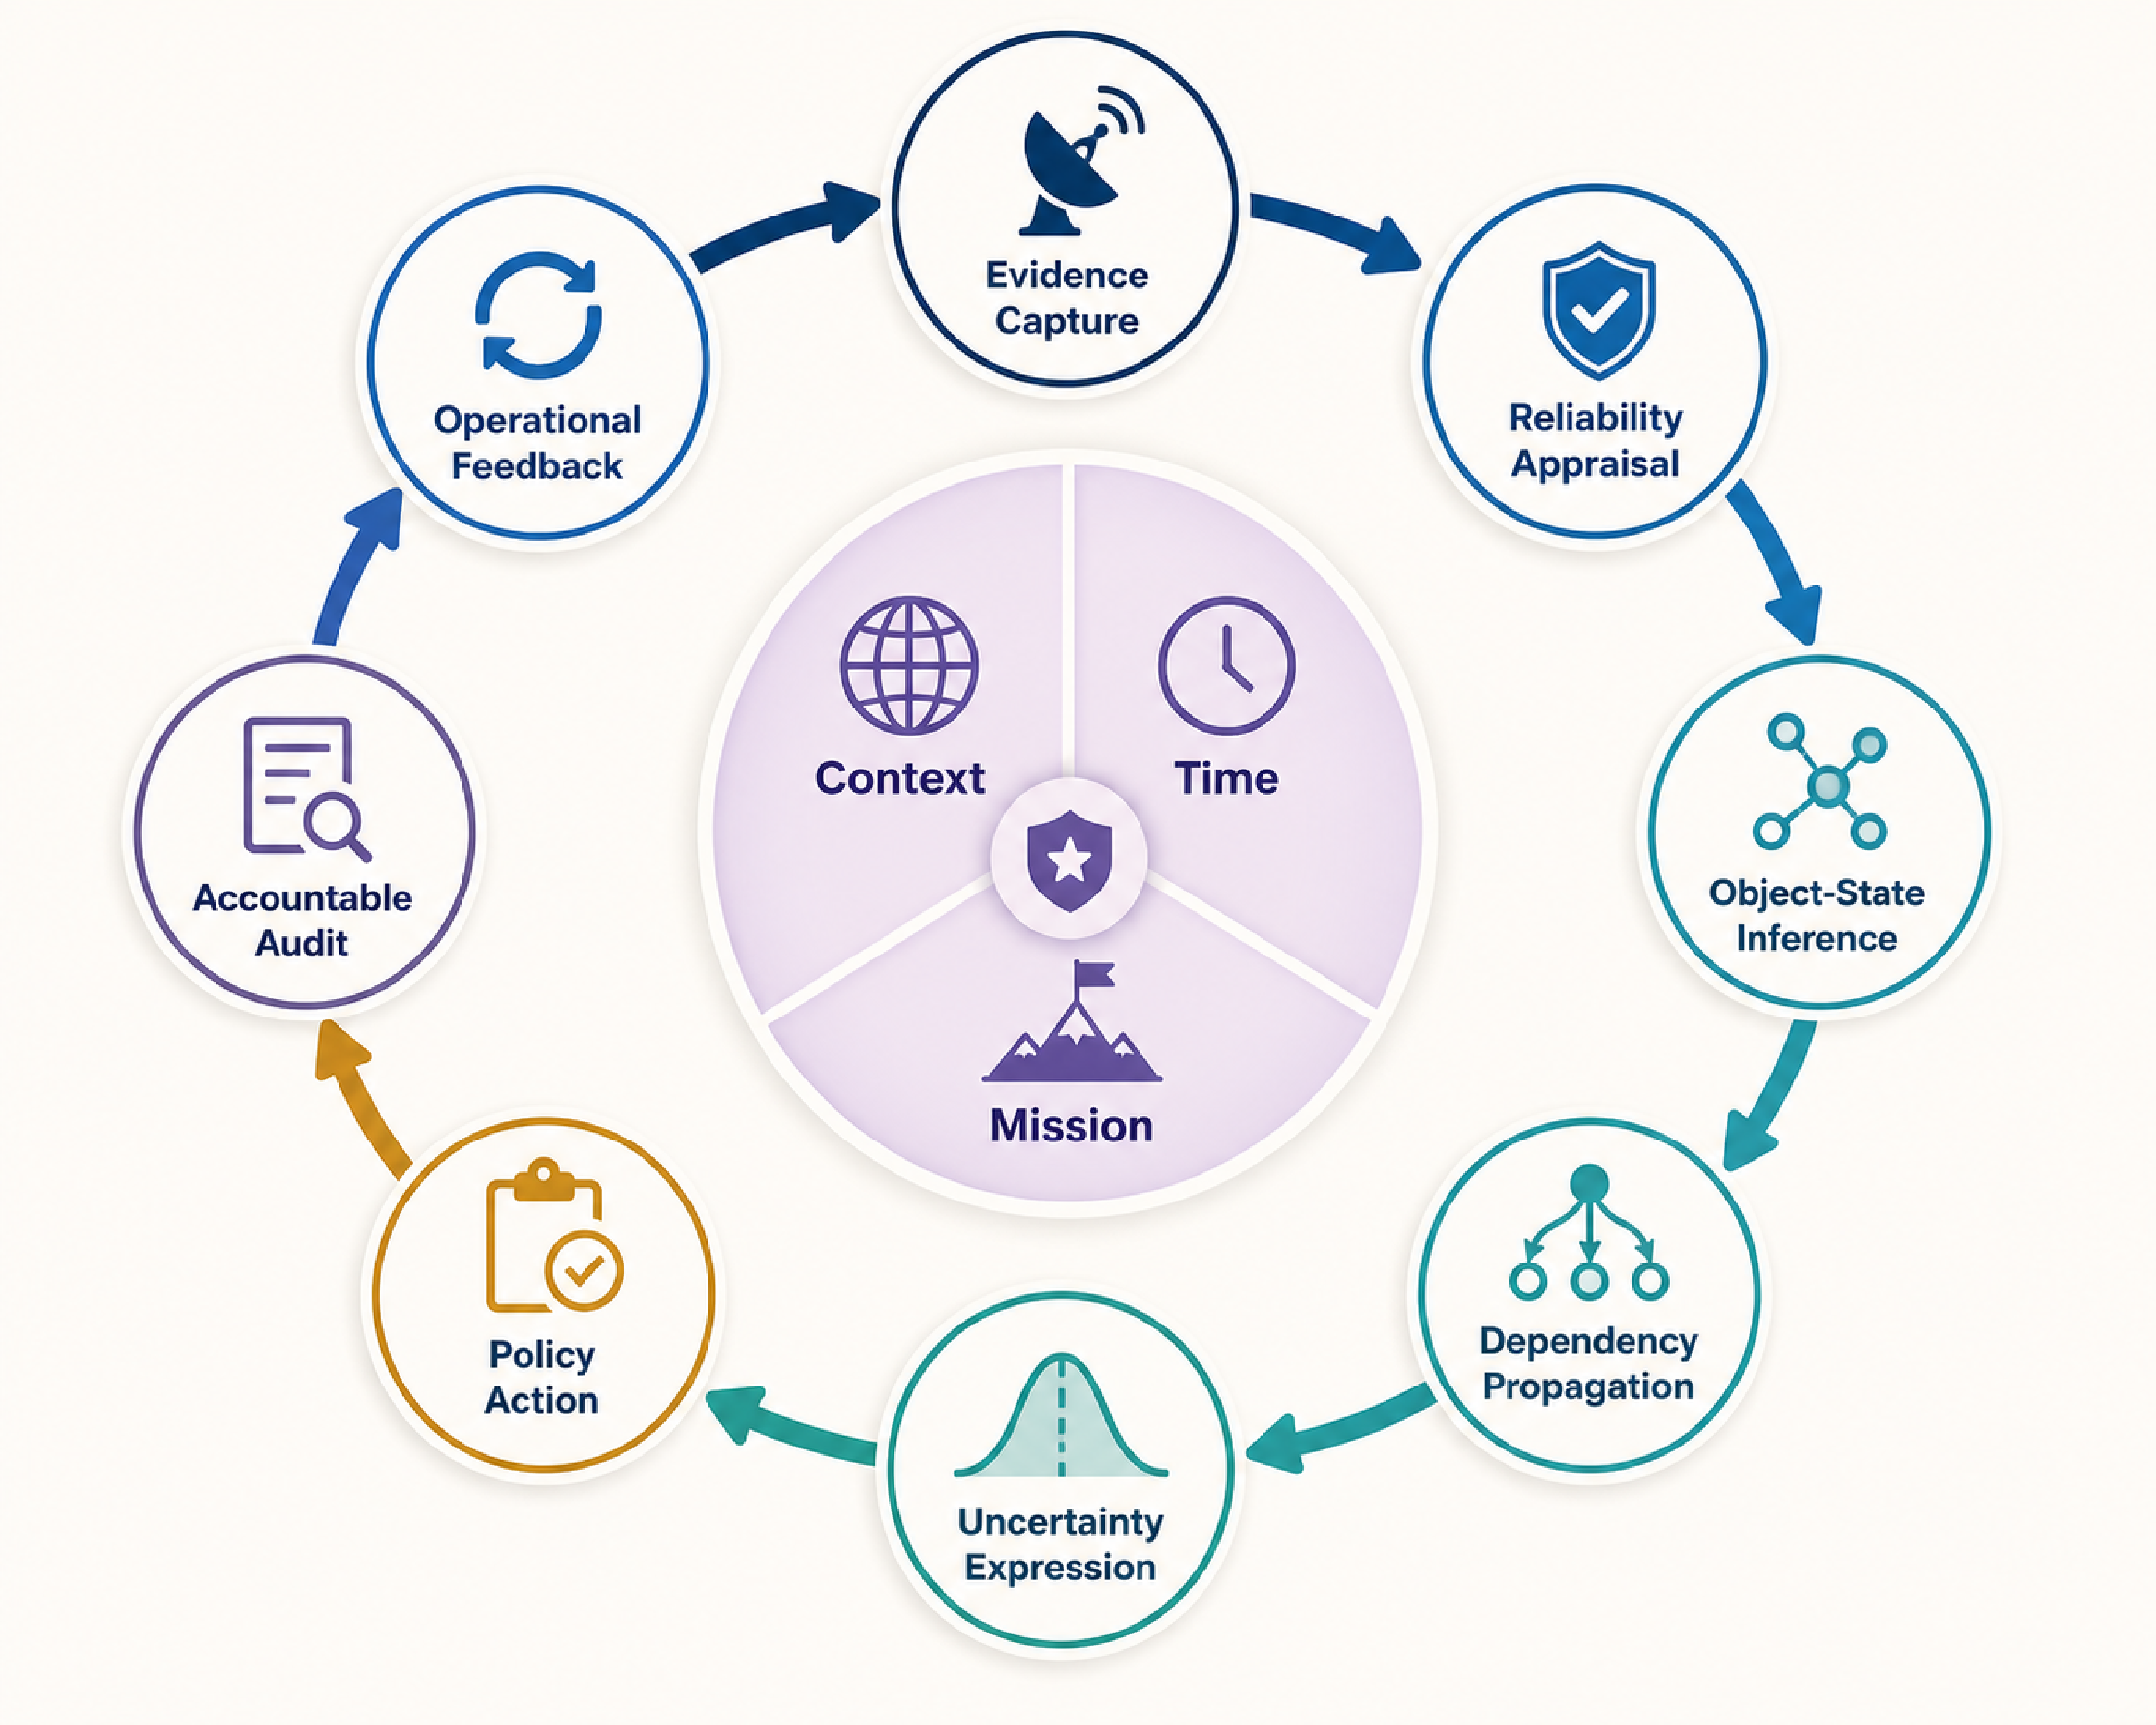
\includegraphics[width=0.86\textwidth]{figures/figure-05-ctg-reasoning-loop.pdf}
\caption{CTG workflow for evidence appraisal, dependency review, uncertainty representation, policy action, and audit. The diagram specifies information flow; performance depends on the selected methods and their mission-specific validation.\label{fig:ctg}}
\end{figure}

Evidence reuse requires special care. A gateway's report can influence device reputation, link assessment, data quality, and a fused decision; treating the resulting scores as independent can count the same observation repeatedly. Implementations retain unique evidence identifiers, parent identifiers, and shared calibration, localization, model, operator, and relay dependencies. Exact duplicates contribute once to a given update. Distinct observations with shared causes require a joint model or a method with stated dependence assumptions; any discounting rule requires justification under those assumptions. For unresolved dependence, a policy may classify the evidence as potentially dependent or request another source. Statistical independence requires assessment of shared navigation references, training data, and environments, including across distinct identities or organizations. Ledger persistence preserves the recorded lineage for appraisal, subject to capture completeness.

\subsection{A Bounded Decision Trace}

A constructed policy example illustrates how a USV gateway assesses a target-location product for UUV route replanning. Its thresholds specify the example; operational use requires mission-specific selection and validation. Policy version $p_7$ requires an unexpired delegation, verified product provenance, an accepted platform appraisal, acquisition age at most $60$ s including clock uncertainty, and corroboration independent of the identified common localization failure. Replanning requires every gate to pass, with freshness and observation validity assessed alongside the ledger commitment.

At decision time, the gateway has a signed observation $d_1$ with an acquisition-age interval of $[42,48]$ s, a fused product $d_2$ whose only observation parent is $d_1$, and an observation $d_3$ from a second vehicle with age interval $[58,66]$ s. The authorization, provenance, and platform-appraisal gates are assumed to pass. The lineage shows that $d_1$ and $d_2$ supply one observation lineage, while $d_3$ uses the same localization reference as $d_1$. The decision trace is then reproducible: $d_1$ passes freshness; $d_2$ reuses the same observation lineage; and $d_3$ exceeds the worst-case freshness bound while retaining the shared localization concern. The gateway records the target-location claim as requiring further support and selects the preauthorized local fallback specified by $p_7$ in place of replanning. The decision rests on evidence sufficiency; attribution of malicious behavior is a separate assessment.

The audit record contains the gate results, lineage identifiers, assessed uncertainty, policy and platform-appraisal versions, delegated-authority basis, and selected fallback. A fresh observation with an adequately justified independent localization basis would trigger reassessment. Observation age and independence retain their acquisition and lineage meanings when ledger inclusion occurs later. This trace makes the framework operational at the level of a reviewable decision procedure while leaving threshold selection, fallback safety, and mission-loss evaluation to an implementation study.

\subsection{Trust Methods and Appropriate Claims}

The literature offers several method families, summarized in Table~\ref{tab:trust-methods}. Each expresses a different claim under different assumptions. The qualitative comparison provides a selection guide for future mission-specific validation.

\begin{table}[!htbp]
\caption{Trust-inference families and their role in CTG.\label{tab:trust-methods}}
\begin{adjustwidth}{-\extralength}{0cm}
\small
\begin{tabularx}{\fulllength}{@{}P{30mm}P{40mm}YYY@{}}
\toprule
\textbf{Family} & \textbf{Useful representation} & \textbf{Strength} & \textbf{Critical assumption/risk} & \textbf{Representative sources}\\
\midrule
Weighted multi-attribute score & Context-weighted evidence features & Interpretable and implementable at constrained edges & Weights and thresholds can be arbitrary or task-insensitive & \citep{ahmed2019trust,aaqib2023iot}\\
Probabilistic trust/reputation & Evidence-updated belief or behavior propensity & Supports sequential assessment when the update model is specified & Priors, dependence, and behavior persistence require justification & \citep{mui2003computational}\\
Subjective logic & Belief, disbelief, uncertainty, and base rate & Makes ignorance visible and supports opinion combination & Dependence and source identity must be handled explicitly & \citep{jsang2016subjective}\\
State-space/Markov & Latent state with temporal transitions & Represents persistence and recovery & State meanings and transition parameters need mission data & \citep{arifeen2020hidden}\\
Rule/tree/fuzzy methods & Human-readable rules or learned partitions & Can combine heterogeneous evidence & Coverage gaps and abrupt boundaries; calibration often unclear & \citep{jiang2020dynamic,zhu2024design}\\
Machine/deep learning & Learned anomaly or multi-view representation & Captures nonlinear patterns & Shift, poisoning, explainability, and overconfidence & \citep{shafique2021detecting,dang2022deep,liu2022trusted}\\
Graph-based propagation & Relational evidence over dependencies & Connects local evidence to downstream exposure & Correlation, cycles, and collusion can amplify error & \citep{kamvar2003eigentrust,bellini2020blockchain}\\
\bottomrule
\end{tabularx}
\end{adjustwidth}
\end{table}

The underwater studies provide concrete examples of these model assumptions and their evaluation conditions. The HMM proposal in \citet{arifeen2020hidden} maps packet-loss rate and packet-error rate to latent malicious/trustworthy states; its MATLAB illustration uses ten observations with randomly initialized probabilities and demonstrates a temporal construction under a synthetic numerical setup. TEUC combines data-, link-, and node-based evidence with a C4.5 tree and reward/penalty updates \citep{jiang2020dynamic}. The study identifies acoustic loss as a reason normal nodes may receive low trust and assumes attack-free initial deployment so that the initial training evidence is unpolluted; its MATLAB simulation is conditioned on that setup. The broader UWSN review identifies evidence collection, evaluation, propagation, and updating as distinct design choices \citep{zhu2024design}. Together, these studies motivate three CTG requirements: keep node behavior distinct from sensor truth, assess attack classification alongside mission decision loss, and retain benign degradation as a possible explanation.

Equation~\eqref{eq:trust} provides an assessment interface for these methods when the output states the assessed property, context, horizon, uncertainty representation, and supporting validation. Probabilities require an event definition and calibration assessment; ordinal scores require an ordering interpretation and justified thresholds. Spectral reputation, such as EigenTrust, expresses relative reputation; its use as a mission-success probability would require an explicit event model and calibration \citep{kamvar2003eigentrust}. The reliance policy separately specifies authority, constraints, and decision consequences. Beta parameters, hidden-state transitions, scoring thresholds, message schemas, and performance targets remain empirical design choices for each implementation study.

\section{Blockchain-Assisted Assurance: Roles and Boundaries}

\subsection{The Decision to Use a Ledger}

The decision to use blockchain begins with the governance structure and required record semantics. A permissioned ledger is plausible when independently administered parties require joint control over accepted state transitions and cannot assign that role to one agreed custodian. Multi-party participation, signatures, or intermittent connectivity alone do not establish that need. A signed append-only log with independent witnesses, an authenticated database with protected audit records, or a jointly administered replicated database may provide the required accountability. The design should state which unilateral changes must be prevented, who can authorize conflicting updates, and which fault model the alternatives must tolerate before comparing their cost. Local verified control serves hard real-time loops.

A permissioned ledger is a plausible choice for the bounded-membership missions considered here because admission and endorsement can follow organizational authority. Permission model and consensus resource cost are separate design choices; permissionless participation does not necessarily imply proof of work. Resource-intensive peers and ordering services can reside on capable shore, edge, or selected USV nodes, while constrained vehicles submit transactions or verify supported proofs under explicit trust assumptions. Hyperledger Fabric provides a representative architecture with identities, endorsement policies, channels, ordering, and validation \citep{androulaki2018hyperledger,hyperledger2026fabric}. Its documentation distinguishes crash-fault-tolerant Raft ordering from Byzantine-fault-tolerant ordering. A Raft deployment does not obtain malicious-orderer tolerance merely from permissioned membership. Ordering, endorsement, and application validation protect different steps; clients must check a valid commit, since inclusion in a block need not mean a transaction updated application state \citep{hyperledger2026fabric}. OAL accommodates another shared-state service when its fault, availability, and governance assumptions match. Consensus surveys describe trade-offs among throughput, finality, membership, energy, and fault tolerance \citep{wang2019survey,lashkari2021comprehensive,zhang2020analysis}.

\begin{figure}[!htbp]
\centering
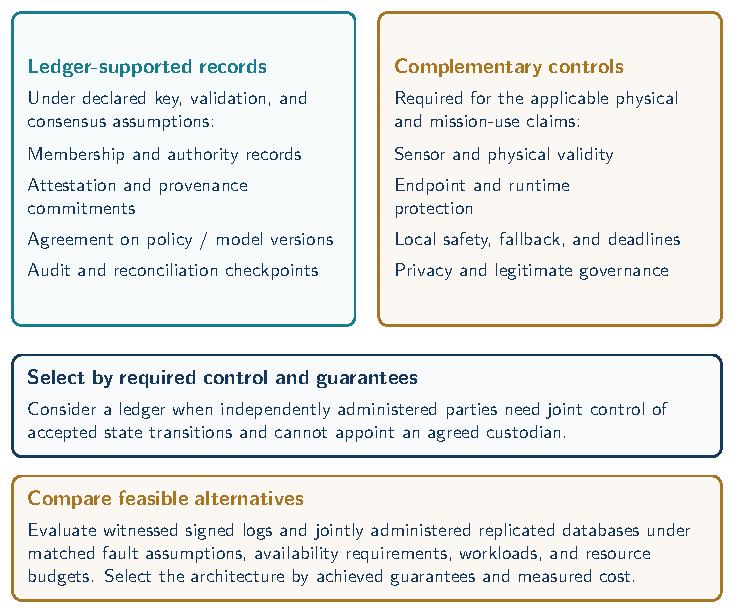
\includegraphics[width=0.92\textwidth]{figures/figure-06-blockchain-boundary.pdf}
\caption{Blockchain boundary in mission trust. Ledger-supported records and complementary controls serve distinct claims. Selection depends on required joint control and comparison with witnessed logs and replicated databases under matched assumptions.\label{fig:blockchain-boundary}}
\end{figure}

\subsection{On-Chain and Off-Chain Partitioning}

Raw video, sonar, point clouds, high-rate telemetry, detailed attestation evidence, and fine-grained location should remain off chain, encrypted and subject to data-use policy. The ledger records small, verifiable references: content identifiers or Merkle roots, producer and custodian identifiers, coarse timestamps or time ranges, schema and policy versions, attestation-result commitments, endorsement decisions, revocations, and audit outcomes. The commitment scheme specifies the exact bytes or canonical representation covered, its algorithm, and whether it commits to plaintext or ciphertext. Storage and retention arrangements preserve authorized access to the corresponding evidence; a digest supplies neither availability nor recoverability. The consumer records the ledger state, local authority information, and time uncertainty available at creation and use. Reconciliation separately evaluates these against subsequently learned events.

On-chain hashes provide integrity commitments. Privacy comes from encryption, access control, selective disclosure, retention rules, key destruction, aggregation, and metadata minimization, because hashes can reveal equality, support dictionary attacks on predictable values, and bind sensitive metadata to a durable member-visible record. On-chain metadata also persists after an off-chain object is deleted. Privacy design therefore accounts for traffic analysis, membership visibility, timing, and the linkage of vehicle identifiers across missions. General IoT and blockchain reviews identify privacy and storage tension \citep{reyna2018blockchain,li2020survey,nguyen2020blockchain}; maritime governance adds commercial and jurisdictional concerns \citep{li2021survey,farah2024survey,zhou2020key}.

\subsection{Five Design Patterns}

Table~\ref{tab:blockchain-patterns} organizes recurring ledger uses by OAL claim, assumptions, and complementary assurance requirements. The patterns synthesize UAV, IoT, provenance, and attestation work into reusable design templates.

\begin{table}[!htbp]
\caption{Blockchain design patterns for cross-domain mission assurance.\label{tab:blockchain-patterns}}
\begin{adjustwidth}{-\extralength}{0cm}
\scriptsize
\begin{tabularx}{\fulllength}{@{}P{30mm}P{35mm}P{40mm}YY@{}}
\toprule
\textbf{Pattern} & \textbf{On-chain record} & \textbf{Assurance supported} & \textbf{Necessary assumptions} & \textbf{Complementary assurance required}\\
\midrule
Membership and authority registry & Organization, role, credential status, delegation and revocation version & Cross-party identity and policy-state consistency & Governed issuer set, protected keys, bounded offline credentials & Real intent, endpoint integrity, emergency authority conflict\\
Attestation anchor & Evidence digest, verifier identity, result, reference-value and policy version & Accountable device-state appraisal and freshness history & Trustworthy measurement root and verifier; adequate coverage & Sensor truth, unmeasured runtime behavior, compromised verifier\\
Provenance commitment & Data/version identifier, transformation and custody roots, endorsement & Tamper evidence for recorded lineage and processing & Adequate instrumentation, bounded time uncertainty, protected keys, retrievable evidence & Semantic correctness, omitted events, biased models, metadata confidentiality\\
Partition-aware audit and reconciliation & Signed sequence range, batch root, local policy/model version, reconnect event & Detectable gaps or conflicts relative to retained checkpoints & Protected append state, independently retained checkpoints, eventual evidence retrieval & Unwitnessed suffix loss, uncaptured events, uncertain event time, physical truth\\
Policy/model coordination & Approved artifact identifier, activation/rollback time, authorized endorsers & Agreement on approved versions among synchronized participants & Governed approval, version validation, activation and rollback rules & Actual deployment state, partitioned participants, artifact safety and performance\\
\bottomrule
\end{tabularx}
\end{adjustwidth}
\end{table}

The membership pattern generalizes UAV identity and authentication proposals \citep{han2022identity,tan2022blockchain,karmakar2024blockchain}. It records which organization may issue each role, the applicable policy version, and how offline parties learn of revocation. Short-lived credentials, bounded delegation, and risk-specific offline envelopes constrain exposure while revocation information propagates.

Two full-text authentication studies provide prototype-level evidence for membership and channel establishment. Tan et al. evaluate Hyperledger Fabric smart-contract operations and cryptographic communication/computation costs in a simulated $10\,\mathrm{km}\times10\,\mathrm{km}$ UAV mission with cloud-hosted peers and assumed base-station coverage \citep{tan2022blockchain}. SwarmAuth combines PUF-based mutual authentication, a blockchain registry, and location-aware clustering, then evaluates security features, computation and communication cost, throughput, and delay using an EVM implementation and simulations \citep{karmakar2024blockchain}. OAL maps these results to entity/platform admission and ledger-supported registry claims. Observation validity, underwater partition behavior, cross-organizational governance, and consequence-weighted mission decisions form the corresponding cross-domain validation extensions.

The attestation pattern links RATS evidence appraisal to shared audit. An attester produces evidence; a verifier evaluates it under an appraisal policy; a relying party appraises the result for its intended use \citep{birkholz2023remote}. Recording a commitment to the result and policy supports later review and comparison of verifier outputs among organizations. Attestation architectures for blockchain and edge systems illustrate this intersection \citep{hardjono2021towards,ott2023universal,figueiredo2022arcadian,baciu2025secure}. Sensitive measurement detail remains encrypted off chain by default. The permitted age of a result is a relying-party policy bound, not a guarantee that device state remains unchanged until expiry; RATS explicitly recognizes the race between appraisal and subsequent state changes \citep{birkholz2023remote}.

Heterogeneous attestation is technically plausible, with platform-specific cost. The hardware-agnostic framework of \citet{ott2023universal} was implemented for TPM, AMD SEV-SNP, and ARM PSA evidence. Its mutual attested-TLS evaluation reported $31.2$ ms for SEV-SNP virtual machines on the same host and $476.1$ ms for the tested Intel firmware TPM, the latter dominated by quote generation. ARM PSA handshake latency was not measured because TLS was not implemented on that embedded device. These configuration-specific results are not a cross-domain communication benchmark. They motivate retaining technology, configuration, freshness, and measurement scope with an attestation result. Measured software identity must also be interpreted against reference values and software assurance evidence; matching an approved image does not demonstrate that it is vulnerability-free or that its sensor observations are accurate.

The provenance pattern links W3C-compatible derivation to shared commitments. IoT provenance proposals use blockchain to protect provenance records or bind large off-chain collections \citep{hang2019design,honarpajooh2021iot,khan2020iot,rahman2020secure}. For mission data, each derived product should identify immutable inputs, transformation code or model, parameters, responsible entity, and output version. Provenance supports explanation and accountability, including for AI artifacts \citep{kale2023provenance}; observation-validity and mission-suitability appraisal assess the semantic quality of the transformation and its output.

The partition-aware pattern is especially relevant to underwater missions. A node or gateway keeps a signed, hash-linked local sequence, retains a batch root locally during disconnection, and submits it with a sequence range and prior checkpoint when connectivity permits. Verifiers check signatures, membership evidence, sequence continuity, duplicates, policy versions, and consistency with independently retained checkpoints. Inclusion proofs establish membership in a committed batch; they do not establish that every physical event was captured. Missing entries inside a known sequence range or conflicting disclosed histories may be detected, while deletion of an unwitnessed suffix can remain invisible. Protected counters, independently held receipts, and explicit capture assumptions determine the strength of the audit claim.

Partition handling separately specifies ledger safety, ledger liveness, and local mission authority. Here, ledger safety means that correct replicas do not finalize conflicting histories under the selected protocol's assumptions; liveness means that eligible requests can progress when its quorum and communication conditions hold. Losing the required quorum can suspend new commits while previously verified records remain locally usable. The CAP result concerns the impossibility of simultaneously guaranteeing linearizable shared read/write state and completion of every request at nonfailed nodes under arbitrary partitions \citep{brewer2000towards,gilbert2002brewer}. It does not require every local mission function to stop or guarantee a real-time deadline. Predelegated local actions can continue within their envelope, but an offline decision that requires fresh global state must wait, use an explicitly weaker state assumption, or follow its authorized fallback. Later reconciliation records conflicts and their disposition; it cannot retroactively make an unsafe physical action safe.

\subsection{Governance, Revocation, and Recovery}

Permissioned consensus places trust in explicit consortium rules. A consortium defines member eligibility, validator distribution, endorsement thresholds, emergency powers, software upgrade, key rotation, data jurisdiction, dispute resolution, incident disclosure, and exit. Multiple replicas controlled by one administrator do not provide independent organizational control of history. Conversely, different organizational names do not establish fault independence if validators share administrators, cloud credentials, software defects, or key custody. The governance assessment therefore identifies who can change membership and policies, override controls, or deny a quorum. Endorsement thresholds and validator placement must be evaluated against that distribution of authority and the required availability.

Revocation is temporal. A credential revoked with effect from 12:00 may have authorized a disconnected UUV's action at 11:55, while the gateway learns the revocation at 12:30. This interpretation requires a declared effective-time rule and trustworthy bounds on the action time; a signed timestamp alone cannot establish when the event occurred. Audit separates event-time intervals, receipt and commitment times, locally known credential status, the applicable delegation, and subsequently learned revocation. If the event-time interval overlaps revocation or key compromise is suspected, the validity finding may remain disputed. Recovery reviews identities, affected models, data products, recorded provenance descendants, device re-attestation, and consequential mission decisions. The ledger and dependency graph help locate the recorded affected set; missing lineage requires additional investigation.

\subsection{Real-Time and Safety Boundaries}

Deadline-bound vehicle functions require local control with timing and safety arguments appropriate to stabilization, collision avoidance, or an emergency maneuver. The ledger can coordinate approved policy or software versions before operation, record summaries afterward, and support slower supervisory decisions, cross-party authorization, data release, and audit. Removing a ledger dependency from a control path avoids making consensus progress a prerequisite for that path, but platform safety still depends on local sensing, control, resources, and the chosen fallback. For example, emergency surfacing must itself be assessed against the local environment. Reduced audit freshness and cross-organizational coordination remain visible during ledger-service loss.

Figure~\ref{fig:blockchain-boundary} provides a claim discipline. Under the configured fault and key assumptions, a ledger supports evidence about accepted endorsements, versions, and record order. Physical, endpoint, timing, privacy, and governance evidence is additionally required to assess whether observations matched the world, endpoints met their integrity requirements, deadlines were satisfied, and authority was appropriate.

\section{Evaluation Practices and Evidence Maturity}

The reviewed sources include conceptual architectures, analytical models, simulations, prototypes, datasets, and domain demonstrations. Each form answers a distinct question: security analysis exposes protocol assumptions; network simulation explores scale; blockchain prototypes measure implementation behavior; and field trials examine integration under specified operating conditions. The framework below organizes these forms for future evaluation of mission-trust claims. It does not estimate their prevalence across the literature or report an integrated evaluation of OAL.

\subsection{A Claim-Specific Evidence Profile}

Figure~\ref{fig:maturity} proposes six complementary evidence categories spanning conceptual work, analysis, and operational experience. The numbering is an organizing convention, not a cumulative quality score: formal analysis, experimental control, environmental representativeness, and operational duration are distinct dimensions. A field trial need not contain a formal proof, and deployment does not establish resistance to an untested adversary. Each claim therefore receives an evidence profile identifying the methods used, system scope, assumptions, and conditions tested; one highest category cannot summarize an entire system.

\begin{figure}[!htbp]
\centering
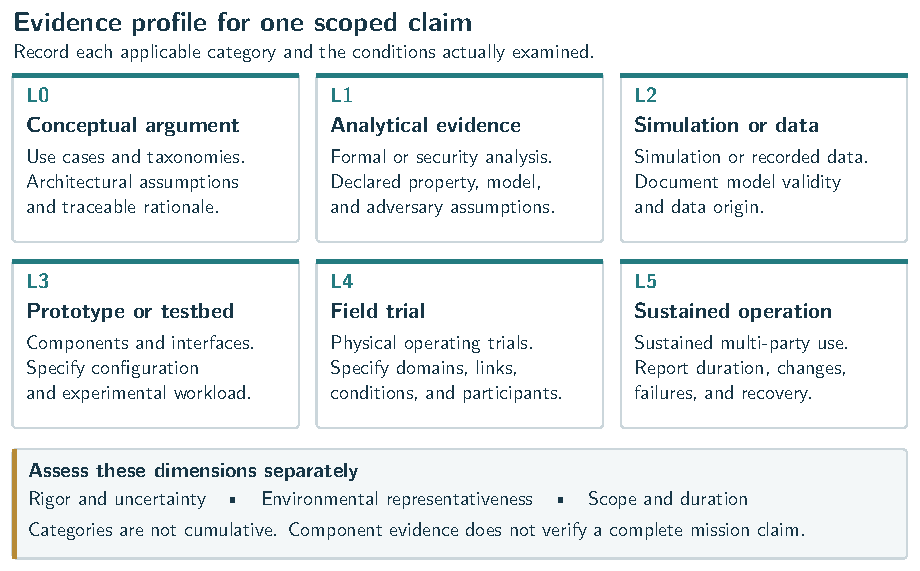
\includegraphics[width=\textwidth]{figures/figure-07-evidence-maturity.pdf}
\caption{Authors' claim-specific evidence profile. The six categories indicate the setting and method supporting a claim; they do not imply cumulative verification or a ranking of scientific rigor.\label{fig:maturity}}
\end{figure}

Category L0 denotes a use case, taxonomy, or architecture supported by conceptual argument. L1 denotes mathematical, formal, or security analysis with explicit adversary and system assumptions. L2 denotes simulation or recorded-data analysis; the origin and representativeness of the data are recorded separately. L3 denotes an implementation tested in a prototype or testbed with a documented configuration and workload. L4 denotes trials under specified physical operating conditions, identifying which vehicle domains, communications, and participants were represented. L5 denotes sustained multi-party operation, with duration and observed governance changes, credential rotation, failures, audits, and recovery reported explicitly. A ledger-throughput test supplies prototype evidence for that component; it does not establish observation validity or mission safety. Integrated claims require evidence for each consequence-relevant dependency, including the interfaces between components.

\subsection{Datasets, Simulators, and Testbeds}

Existing public resources provide candidate components for a cross-domain evaluation environment. TON\_IoT combines labeled IoT/IIoT telemetry, operating-system logs, and network traffic collected in the UNSW Canberra cyber range; Edge-IIoTset uses a purpose-built seven-layer testbed and supplies baselines for centralized and federated learning \citep{alsaedi2020ton,ferrag2022edge}. Together with CICIoT2023 \citep{neto2023ciciot2023}, they support device/link anomaly experiments. Transferring these experiments requires a separate model of maritime topology, physical degradation, and mission consequence. SeaDronesSee provides maritime UAV imagery and metadata for visual detection and tracking experiments \citep{varga2022seadronessee}; evaluating observation validity additionally requires defined physical claims and appropriate ground truth. The supervised GNSS study of \citet{semanjski2020use} trains on synthetically manipulated signals and validates on two distinct real-world spoofing/meaconing datasets, contributing evidence for the evaluated signal features and recording contexts.

The original AirSim study describes a high-frequency physics engine, visual environments, and real-time hardware-in-the-loop support, with selected software components compared against real flights \citep{shah2018airsim}. UUV Simulator extends Gazebo/ROS with hydrodynamics, thrusters, sensors, external disturbances, and multi-robot scenarios \citep{manhaes2016uuv}, while Aqua-Sim NG ports underwater-network functionality to ns-3 and evaluates the redesigned simulator architecture \citep{martin2017aqua}. These resources address complementary components: air-domain perception and dynamics, underwater robot simulation, and underwater communication protocols. Coupling them is proposed integration work, requiring compatible software versions, time synchronization, shared geometry, validated channel interfaces, and reproducible event exchange. Attestation, provenance, consortium behavior, and mission-loss modules must also be implemented and validated; combining the tools alone supplies no ground truth for those claims.

\begin{table}[!htbp]
\caption{Evaluation resources and transfer limits. OAL uses and metrics are proposed evaluation requirements, not results established by each resource.\label{tab:evaluation}}
\begin{adjustwidth}{-\extralength}{0cm}
\scriptsize
\begin{tabularx}{\fulllength}{@{}P{33mm}P{34mm}P{40mm}YY@{}}
\toprule
\textbf{Resource/practice} & \textbf{Primary evidence} & \textbf{OAL use} & \textbf{Important metrics} & \textbf{Required complement}\\
\midrule
CICIoT2023, TON\_IoT, Edge-IIoTset & Labeled network, host, sensor, and attack telemetry; centralized/federated baselines & Device/link anomaly and uncertainty methods & Detection by class, calibration, false isolation, delay, missingness sensitivity & Cross-media maritime topology, physics, and mission-loss model\\
SeaDronesSee and GNSS records & Real maritime imagery/metadata and real-world signal-manipulation records & Observation validity, data-product quality, spoofing context & Detection error, geolocation error, uncertainty calibration, robustness to weather/viewpoint & Underwater, ledger, and additional observation contexts\\
AirSim & High-frequency physics, sensors, visual worlds, hardware-in-the-loop & Air-domain observation and mission use & Mission success, safety constraint violations, sensor/model shift & Acoustic-network and consortium-governance modules\\
UUV Simulator & ROS/Gazebo hydrodynamics, thrusters, sensors, disturbances, multi-robot scenarios & Underwater motion, sensing, control, integration & Localization, energy, mission completion, failure recovery & Field validation of hydrodynamics and sensor behavior\\
Aqua-Sim NG/ns-3 & Underwater-network protocols, channel abstractions, routing experiments & Link/path evidence, delay, loss, routing and partition & Delivery, latency distribution, energy, path churn, outage duration & Physical observation-validity module\\
Permissioned-ledger testbed & Peers, ordering, endorsement, contracts, failures & Ledger/governance consistency and audit & Commit/finality latency, throughput, resource use, recovery, fork/conflict handling & Representative evidence sizes, event rates, and duty cycles\\
Cross-domain field exercise & Physical platforms, operators, weather, real links & Integrated lifecycle and mission-use suitability & Consequence-weighted mission outcomes, false quarantine, recovery time, audit completeness & Repeatable scenarios and systematic adversarial coverage\\
\bottomrule
\end{tabularx}
\end{adjustwidth}
\end{table}

\subsection{Metrics that Respect the Assurance Chain}

An integrated mission-trust evaluation should cover five metric families. First, \emph{inference quality}: discrimination where labels exist, calibration for probabilistic outputs or coverage for uncertainty intervals, uncertainty under missing evidence, detection and recovery delay, and performance under distribution shift. Accuracy alone is inadequate because a rare false isolation can remove a critical relay. Second, \emph{mission effect}: task completion, time, coverage, safety-constraint violations, decision regret, and resource allocation under adversarial and benign degradation. Third, \emph{network cost}: bytes per evidence event, delay distribution rather than only mean delay, energy, storage growth, duty cycle, and partition duration. Fourth, \emph{ledger behavior}, where a ledger is used: endorsement and finality latency, throughput under realistic event batching, validator/resource cost, membership change, outage behavior, reconciliation completeness, and disputed histories. Fifth, \emph{accountability}: percentage of decisions with resolvable provenance, time to determine affected descendants, policy/model version traceability, and successful revocation and recovery.

Experimental factors should cross object, threat, and context dimensions. Examples include compromised entities versus devices; isolated versus colluding nodes; jamming versus environmental fading; fresh versus stale attestation; independent versus correlated sensors; honest versus compromised gateways; short versus prolonged partitions; and routine versus high-consequence mission policies. A factorial or explicitly sampled scenario design can test their interactions. Ground truth should distinguish nominal operation, benign degradation, and adversarial intervention, including cases where they coexist. Missing or ambiguous evidence is a separate observation condition, and ``unknown'' is an inference outcome. Attack labels in a benchmark do not themselves validate attribution in an operational environment.

Training, threshold selection, calibration, and final evaluation should use separate data. Splits should respect shared recording episodes, platforms, sites, and time periods where these could leak information between partitions. Comparisons should use paired scenarios, with uncertainty intervals based on independent missions or simulation runs rather than treating correlated packets as independent replications. Report class prevalence, per-condition outcomes, the frequency and cost of abstention, and sensitivity to mission-loss weights. Latency summaries should include deadline misses and undelivered events so that low delay among successful deliveries does not conceal loss of availability.

Baselines should also be layered. An authenticated centralized database and signed append-only logs test whether shared ledger state adds value for the stated governance problem; independently witnessed or replicated signed logs provide a stronger comparison where parties distrust one administrator. Removing replication, continuous appraisal, lineage, dependency handling, or explicit uncertainty in separate ablations can isolate their contributions. Comparisons should use the same application workload, evidence, access requirements, resource budget, and attacker capabilities. Architecture-specific mechanisms such as endorsement need not be identical, but differences in trust assumptions and achieved guarantees must be stated. Each method should receive a comparable tuning budget and feasible operating configuration. Studies of Fabric-based access control and integrated IoT ledgers offer implementation starting points \citep{liu2020fabric,hang2019design}, completed by application-specific baselines.

Reproducibility requires the exact topology, channel and mobility models, workload, cryptographic settings, software releases and configuration, endorsement and fault model, random seeds, data partitions, trust-policy versions, and mission-loss function. Versioned provenance should cover the evaluation itself. If a policy threshold or model changes between runs, the reported outcome belongs to a different system configuration and assurance claim.

\subsection{Interpreting Claims by Evidence Profile}

UAV blockchain applications range from security and privacy architectures to swarm monitoring and resilient-network proposals \citep{ch2020security,xiao2021blockchain,abualsauod2022hybrid,garcamagario2019security,zhou2024towards}. A maturity classification requires inspection of the particular claim and its evaluation, rather than inference from the application label. Broader work on Industry 4.0, federated learning, digital twins, supply chains, and government sharing supplies organizational patterns for comparison \citep{javaid2021blockchain,javed2022integration,suhail2022trustworthy,kshetri20181,lnes2017blockchain}. Their applicability to cross-domain missions remains conditional on endpoint, link, timing, governance, and mission-consequence evidence under intermittent connectivity.

The supplementary records distinguish bibliographic inclusion, local full-text availability, screening, and completed claim-level coding. Sixteen sources have completed claim-level coding for the detailed comparisons in this version. These workflow counts do not estimate research maturity or effectiveness. Completed coding supports comparisons within its recorded scope; entries awaiting inspection or coding identify outstanding evidence work. The matrix therefore supports traceability while leaving a corpus-wide maturity distribution undetermined.

\section{Discussion and Research Agenda}

\subsection{Theoretical Implications}

OAL represents trust as a structured relying relation. This yields three design implications. First, assurance arguments can be composed through typed dependencies when their inference rules and shared assumptions are explicit. Entity evidence supports authorization claims, device attestation supports claims about measured state, and observation and mission evidence support downstream use. Formal composition requires a theorem with explicit rules and assumptions for the combined claims. Second, trust is purpose-bound. Evidence sufficient for sharing low-sensitivity imagery may be insufficient for cooperative navigation, even when the underlying object is identical. Third, uncertainty requires an operational response: ``unknown'' records insufficient support for a conclusion and maps to a documented policy action. This epistemic status is represented separately from physical compromise and degradation.

The assurance chain also clarifies the relationship between provenance and truth. Provenance is an argument about history: who generated an artifact, through which activities, from which inputs. Observation validity is an argument about the world. Ledger consistency is an argument about shared records. Mission suitability is an argument about consequence. These claims require separate tests even when they share evidence or failure causes. Provenance and decision-accountability research supports traceable transformations \citep{singh2019decision,kale2023provenance}; OAL makes explicit the mission consumer's judgment about which history supports which use.

\subsection{System Resilience under Partition and Degradation}

Future architectures should treat partition as a routine operating mode. Local policy envelopes require bounded capability, expiry, evidence-age limits, safe fallback, and explicit records of which global facts were unavailable. Reconnection combines synchronization with semantic reconciliation: the system determines which policy was locally available at event time, when a revocation became effective, which dependent claims require reassessment, and whether conflicting observations require mission review. Authorization under a previously delegated envelope and compliance with subsequently learned global state are distinct questions. Blockchain scalability reviews examine throughput and storage among other constraints \citep{hafid2020scaling,khan2021systematic}; cross-domain missions also require explicit treatment of long disconnection, sparse contacts, and consequence-sensitive local autonomy.

Resilience also requires functional diversity. If the USV is simultaneously acoustic gateway, time source, fusion node, policy-enforcement point, and validator, redundant vehicle count can conceal a shared failure dependency. The graph identifies vertices that support many mission paths; quantifying failure probability or mission loss additionally requires reliability and consequence models. Future work should compare architectural redundancy (multiple instances) with evidential independence (different roots, media, sensors, and organizations). Two reports relayed through one gateway share transport and availability dependencies. Independently signed source observations may retain distinct origin evidence; whether the gateway can also alter or bias their interpretation depends on end-to-end protection, selection, and transformation roles.

\subsection{Governance, Privacy, and Human Authority}

Consortium governance is part of the security mechanism. Research should specify who can admit validators, approve reference values, activate contracts and models, invoke emergency powers, decide disputes, and audit the auditors. Maritime blockchain adoption studies already identify policy and organizational factors beyond technical performance \citep{yang2019maritime,zhou2020key,farah2024survey}. In mission assurance, a governance failure can propagate like a cyberattack: an unsafe reference value makes compromised devices appear healthy, or a delayed revocation keeps stale authority active.

Privacy questions extend beyond encrypting payloads. Cross-mission identifiers, validator endorsements, timing, route custody, and model-use records can reveal organizational relationships or vehicle activity. Work on blockchain and IoT warns of immutable metadata and access-control tension \citep{ali2019applications,reyna2018blockchain,kshetri2017can}. Future designs should evaluate unlinkability, data minimization, selective disclosure, authorization-policy confidentiality, and deletion semantics alongside audit value. A mission may need accountable pseudonymity: an operator can verify that an authorized role acted while the long-term identity remains protected, and a governed process can resolve accountability after an incident.

Human authority must remain explicit. Automated trust inference can recommend reduced privilege, corroboration, or isolation, while high-consequence recovery and dispute decisions may require human review. The relevant evidence comprises model output, explanation, policy version, uncertainty, alternatives, and consequence. Authorized and auditable human override preserves this evidence trail and the accountability of the relying decision.

\subsection{Testable Research Propositions}

The following hypotheses translate the synthesis into comparisons for future studies. Each test requires a declared mission distribution, threat model, implementation, primary outcome, and minimum practically meaningful effect. Counterexamples and null effects delimit the conditions under which the proposed structure is useful.

\textbf{P1 (assurance separation).} In matched scenarios containing correctly signed but physically invalid observations, an implementation retaining separate observation, provenance, ledger, and mission-suitability assessments will have a lower unsafe-acceptance rate than a single-score implementation at a matched false-isolation cost. Both receive the same raw evidence, action set, and tuning budget. The outcome is the fraction of invalid products accepted for a specified consequential use, evaluated against an independent physical reference.

\textbf{P2 (dependency awareness).} For a specified binary event and prediction horizon, a probabilistic implementation that models shared sensor and recommender causes will have lower calibration error under correlated error and collusion than its conditional-independence ablation. Both use the same evidence and separately fitted parameters. Evaluation uses a prespecified estimator of held-out calibration, a proper scoring rule such as the Brier score, and decision loss, with results reported across correlation strengths and levels of lineage completeness. The test applies to outputs with an explicit probabilistic meaning.

\textbf{P3 (diagnosis and uncertainty).} Under mixed nominal operation, environmental degradation, adversarial intervention, and evidence outages, an implementation retaining competing causal hypotheses and an explicit unknown outcome will achieve lower prespecified mission loss than a binary trusted/untrusted implementation. Both have access to the same evidence and operational actions. Separate ablations of causal diagnosis and the ability to abstain distinguish their contributions. The loss function includes corroboration delay, false isolation, unsafe acceptance, and lost availability, allowing the effects of diagnosis and response policy to be assessed separately.

\textbf{P4 (bounded offline authority).} Across prespecified partition durations and revocation schedules, bounded offline authorization will complete more permitted tasks before their deadlines than authorization that requires current global approval, and will incur fewer actions conflicting with effective global policy than unrestricted offline autonomy. Both outcomes and resource costs are reported as a trade-off curve over envelope duration and scope. Event-time local authorization and conflicts discovered after reconnection are evaluated separately, using explicit revocation-effective times and clock uncertainty.

\textbf{P5 (selective ledger value).} Under administrator equivocation or record withholding within a declared fault and network model, a permissioned ledger with independent validators will provide more complete, mutually verifiable audit histories than a single-administrator signed log. The comparison measures the fraction of previously accepted test events recovered, detection of inconsistent views, and time to establish an agreed history, using an independent event record as ground truth. A witnessed or replicated signed-log baseline tests whether any gain requires the ledger architecture. Communication cost and deadline misses are measured separately; substantive governance disputes require their own resolution procedures alongside record agreement.

\textbf{P6 (evaluation coverage).} A system configuration selected using transaction and network metrics alone will have higher held-out mission loss than one selected from the same candidates using observation, endpoint, governance, and mission outcomes in addition to those metrics. The comparison uses equal evaluation budgets, fixed selection rules, and paired held-out scenarios containing both benign and adversarial failures. The measured difference tests whether the added evaluation dimensions improve selection for that mission distribution.

Each comparison requires prespecified operating thresholds and analysis rules, effect sizes with uncertainty intervals, and reporting of null or adverse outcomes. Findings apply to the tested implementation and mission distribution; broader applicability requires evaluation across additional configurations and settings.

\subsection{From OAL Cells to an Assurance Case}

OAL can structure an assurance case when each high-consequence mission use is expressed as a scoped claim. For example, ``fused product $d_{17}$ is suitable for route replanning by consumer $r$ until time $t$ under weather class $w$ and policy $p$.'' The argument links that claim to required evidence across the layers. Observation subclaims identify the sensors, calibration, geometry, environmental model, residuals, and corroboration that support physical plausibility. Commitment subclaims identify protected input versions, producers, transformations, custody, and time. Where shared ledger state is required, ledger subclaims state membership, endorsement, ordering, and the agreed policy version. Mission subclaims connect freshness and uncertainty to an explicit consequence and permitted action. Missing support is recorded as an evidence gap; counter-evidence or a challenged assumption is recorded as a potential defeater. Both may justify restricting action, but their epistemic meanings differ.

This structure records both supported scope and boundary conditions. A verifier may establish that a measured software component matches an approved reference, with camera alignment and operator intent assigned to separate subclaims. A provenance record may establish the instrumented derivation path and identify a legacy transformation as a gap in completeness. A ledger may establish endorsement of a model version by three authorized peers, while safety and accuracy are supported by separate validation evidence. Pairing each guarantee with its conditions gives downstream consumers the exact scope of justified reliance.

Assurance cases must also be time-aware. Evidence has an observation time, issue time, receipt time, and expiry condition; a dependency can change between them. If a USV attestation is fresh when it receives a UUV batch but stale when it transforms and endorses that batch, the later activity requires an explicit continuity assumption or renewed evidence. Clock uncertainty is represented where GNSS is unavailable or suspected. For disconnected operation, the case records the last globally known policy and the local authorization envelope, preserving the scope of agreement available at event time.

Counter-evidence is first-class. A new sensor residual, revocation, incident report, or conflicting custody event should identify which claims and descendants become disputed. This enables proportional response: quarantine a derived track while preserving independently supported observations from a platform, or reduce a gateway's endorsement role while retaining its emergency relay function. Recovery closes the argument through review of affected credentials, software, models, data descendants, and mission decisions, producing a scoped and evidence-backed return to service.

Future tools could generate these arguments from the typed dependency graph while preserving human judgment. Policy authors decide evidence sufficiency, independence, consequence, and acceptable uncertainty. The generated artifact therefore distinguishes machine-verified bindings (signature, hash, sequence), verifier appraisals (measured state against reference), statistical assessments (calibration or anomaly), and governance judgments (waiver, dispute, emergency authority). A reviewer can then compare the conclusion with the strongest supported subclaim.

Finally, evaluation should measure the assurance case itself. Evidence coverage can be assessed over an independently reviewed set of consequence-relevant dependencies, with critical gaps reported individually alongside aggregate coverage. Seeded counterexamples test sensitivity to invalid arguments; formal soundness requires a proof under the stated inference rules. Operator studies can measure the time and error in identifying affected products; governance exercises can measure unresolved conflicts and time to an authorized decision. These measures complement detection and ledger performance by testing whether the structure helps users reach appropriately scoped relying decisions.

\subsection{Toward a Cross-Domain Unmanned Trust Profile}

The proposed \CDUTP{} is an agenda for an interoperability profile: a small, versioned set of claims and evidence references for OAL boundaries shared by organizations. Its development agenda covers the schema, protocol bindings, and conformance tests. NIST Zero Trust Architecture supplies resource- and request-centered policy principles \citep{rose2020zero}; IETF RATS supplies attestation roles and semantics \citep{birkholz2023remote}; W3C PROV-DM and PROV-O supply entity--activity--agent provenance relations \citep{w3c2013provdm,w3c2013provo}. NIST's IoT device baseline informs endpoint capabilities \citep{fagan2020iot}. 3GPP specifications for UAS support and maritime services provide communications and service context \citep{threegpp22125,threegpp22119}. Permissioned-ledger governance and endorsement provide candidate mechanisms for multi-party state coordination \citep{androulaki2018hyperledger,hyperledger2026fabric}. Conformance and interoperability require version-specific mappings and tests across the referenced architectures and specifications.

Software update evidence can reuse secure-update architecture. The IETF SUIT architecture describes manifests, authorization, payload acquisition, installation, and device constraints \citep{ietf2020suit}; CDUTP could reference an update identifier and installation result while keeping the firmware payload off chain. Applying similar bindings to learned models would additionally require model-specific compatibility and validation evidence. These mappings would connect domain claims to the mission assurance graph while preserving the scope of the underlying protocol guarantees.

A profile instance should minimally state: object identifier and type; claim and assurance layer; issuer and relying role; evidence or provenance reference; observed, issued, and expiry times; mission context and permitted use; uncertainty or appraisal outcome; applicable policy, model, schema, and contract versions; privacy label and disclosure conditions; parent dependencies; revocation reference; and on/off-chain binding. It should support disconnected issuance and later verification while labeling freshness at the relying time. Compact encodings are desirable for acoustic links, but semantic equivalence is more important than one wire format.

A staged standardization pathway begins with published use cases and claim-scope requirements, followed by a shared vocabulary and conformance tests for evidence lineage and version binding. Subsequent stages comprise plugfests across independently implemented UAV, USV, UUV, gateway, verifier, and ledger components; multi-organization privacy and governance evaluation, including member exit and disputed recovery; and alignment with relevant standards bodies. CDUTP provides a research agenda for that alignment.

\subsection{Design Heuristics}

Several design principles follow from the synthesis. Technology selection begins with the relying decision, object, and assurance claim, which define the roles of the trust method and shared-state service. Evidence management preserves evidence identity and common-cause information, stores raw evidence off chain, minimizes metadata, and explicitly represents staleness and unknown status. Architectures separate hard real-time safety from shared audit and treat policies, models, contracts, and reference values as versioned artifacts exposed to threats. Evaluation includes signed-log and replicated-database alternatives. Descriptions such as ``proposed,'' ``analyzed,'' ``simulated,'' ``prototyped,'' ``field-tested,'' and ``deployed'' identify distinct forms of support, with claim scope stated for each.

These heuristics guide technology selection. Signed append-only logs and replicated databases are candidate solutions when one accountable manager governs state and audit. Distributed agreement may be useful when independent parties require a common history, subject to the fault model, availability constraints, and comparison with independently witnessed logs. Evidence commitments require adequate key custody, time or sequence guarantees, and protected local state. Decisions with deadlines shorter than end-to-end communication require a local safety mechanism whose assumptions and fallback behavior are validated separately.

Responsible deployment adds one final boundary. Mission-trust infrastructure can improve safety, environmental observation, inspection, disaster response, and coalition accountability, while persistent identities and provenance traces also create surveillance and operational-security consequences. An assurance case should therefore include a legitimate-purpose claim, proportional data collection, retention and disclosure limits, and an accountable path for human appeal or incident review. Dual-use assessment focuses on capabilities and governance. Public reporting can disclose architecture, assurance semantics, failure modes, and evaluation methods while protecting credentials, exact operational configurations, exploitable topology details, and mission-specific tactics. This balance supports scientific testing and responsible dissemination. It also reinforces the core OAL insight: governance artifacts and privacy policies are versioned, contestable evidence within the mission system and require the same accountable appraisal as technical artifacts.

\section{Scope and Applicability of the Review and Framework}

The review's conclusions concern the mechanisms and operating conditions represented in the cited literature. Differences in platform, threat model, workload, and evaluation outcome limit direct performance comparisons across studies. The synthesis supports architectural comparisons and conditional design recommendations; it does not establish the prevalence of particular methods or provide pooled estimates of their effectiveness.

UAV security, IoT reputation, road-vehicle trust, industrial provenance, and permissioned enterprise ledgers provide candidate mechanisms for cross-domain transfer. Their threat distributions, time scales, connectivity, energy, and governance define the conditions for comparison with air--surface--underwater operations. The synthesis identifies these transfer assumptions at the conceptual level. Target-environment validation is required to establish performance under the acoustic conditions and operational practices of a particular maritime deployment.

OAL, the dependency relation set, CTG loop, evidence profile, hypotheses, and CDUTP form a conceptual architecture for mission-trust analysis. Integrated implementation, formal composition analysis, and mission experiments provide the evaluation pathway for safety, calibration, availability, and audit-performance claims. Evaluation of the four object types should address coverage and consistent application across settings. Practical graph implementations require rules for abstraction, correlation, privacy, evidence expiry, cycles, and conflicting claims, together with measured computation and communication costs. The general assessment $T_o(t,c,m)$ accommodates several representations; a probabilistic implementation requires a defined event and horizon, an explicit statistical model, and calibration under relevant operating conditions.

The evidence categories organize complementary forms of support, with scope and rigor assessed for each claim. Tests of the research hypotheses require concrete comparators, loss functions, and scenario distributions to determine architectural trade-offs and effect sizes. Development of the CDUTP proposal entails a normative schema, interoperable implementations, and a conformance test suite. Formal analysis, controlled studies, field evidence, and multi-party governance exercises provide complementary support for assessing these contributions.

Finally, the public-evidence focus supports reproducible analysis of assurance, resilience, audit, and responsible governance in civil and publicly documented defense-support settings. Sensitive operational details remain within the governance and disclosure controls of the organizations that hold them. Future authorized studies can evaluate the framework under additional contested-environment and platform-specific conditions.

\section{Conclusions}

Air--surface--underwater cooperation turns trust into an end-to-end mission problem. A defensible decision integrates a plausible observation, an intact and accountable provenance chain, a correctly governed shared state where one is needed, and evidence that remains suitable for the particular mission consequence. The authors' OAL framework connects these four assurance layers to entity, platform/device, link/path, and data-product objects over the complete lifecycle from admission to recovery.

The proposed object-dependency graph and CTG loop organize evidence flow, shared failure causes, uncertainty, and policy action across that structure. They distinguish competing explanations of system behavior from insufficient evidence and require numerical assessments to state their meaning and support. The evidence profile identifies complementary forms of analysis, implementation, environmental testing, and operational experience without treating them as a cumulative quality score.

Blockchain is a candidate coordination mechanism where independent organizations need shared membership and version state, attestation and provenance commitments, accountable audit, and post-partition reconciliation. Its value depends on governance, fault assumptions, and measured costs relative to signed logs and replicated databases. Physical corroboration supports observation validity; attestation appraises measured endpoint state; local safety mechanisms address communication outages and deadlines; and privacy and governance require additional controls. None of these component guarantees alone establishes mission suitability.

The proposed CDUTP and six research hypotheses define work toward interoperable, testable systems. The contribution of this review is the structure of the assurance questions and their connection to selected evidence; performance benefits remain to be established. The next stage combines formal analysis, cross-domain testbeds, representative field trials, and multi-party governance exercises, measuring both decision consequences and the quality of the supporting evidence. The practical objective is to make each consequential mission use traceable to current, appropriately scoped assurance and explicit residual uncertainty.


\vspace{6pt}
\supplementary{The following supporting information accompanies the submission: Table S1, the evidence inventory and analytical coding status (CSV); Table S2, the full-text acquisition and coding manifest (CSV); Supplementary Note S3, discovery queries, status definitions, and source locators (Markdown); and the publication figure files for Figures 1--7 (PDF).}
\authorcontributions{Author contribution details are withheld for double-anonymous review and will be supplied after peer review using the CRediT taxonomy. All authors will confirm that they have read and agreed to the published version of the manuscript.}
\funding{Funding information is withheld for double-anonymous review and will be supplied after peer review.}
\institutionalreview{Not applicable.}
\informedconsent{Not applicable.}
\dataavailability{No new experimental or observational mission data were generated. The supplementary inventory records the literature sources, analytical routing, full-text availability, and coding status used in this narrative synthesis. Source locators support the selected detailed comparisons; title-derived fields serve discovery and routing purposes.}
\acknowledgments{The authors thank those who provided constructive feedback during the preparation of this manuscript.}
\conflictsofinterest{The authors declare no conflicts of interest.}

\Needspace{55mm}
\abbreviations{Abbreviations}{%
\begin{tabular}{@{}ll}
AUV & Autonomous underwater vehicle\\
CDUTP & Cross-Domain Unmanned Trust Profile\\
CTG & Context--temporal--graph\\
DLT & Distributed ledger technology\\
OAL & Object--Assurance--Lifecycle\\
RATS & Remote ATtestation procedureS\\
UAS & Unmanned aerial system\\
UAV & Unmanned aerial vehicle\\
USV & Unmanned surface vehicle\\
UUV & Unmanned underwater vehicle\\
ZTA & Zero trust architecture
\end{tabular}}

\begin{adjustwidth}{-\extralength}{0cm}
\reftitle{References}
\bibliography{references}
\end{adjustwidth}
\end{document}
